\documentclass[
    paper=a4,
    ngerman, % neue dt. Rechtschreibung
    bibliography=totoc,
    headheight=60pt,
    captions=tableheading % Tabelleüberschriften und richtiger Abstand
]{scrartcl}

\usepackage[ngerman]{babel, varioref}
\usepackage[T1]{fontenc} % font encoding for german
\usepackage{lmodern} % Schriftart für Schrift Encoding
\usepackage[utf8]{inputenc} % input encoding
%====Kopfzeile====
\usepackage{scrlayer-scrpage}
\pagestyle{scrheadings}
\clearpairofpagestyles
\usepackage{multicol}

%==============================
%	Mathematikumgebung
%==============================
%====sorgt für bold math symbols, wo sie seien sollten bzw nicht seien sollten;	 ===========
%====keine schöne Lösung, weil siehe Link										 ===========
%(https://latex.org/forum/viewtopic.php?t=4653#top)
\makeatletter
\DeclareRobustCommand*{\bfseries}{
	\not@math@alphabet\bfseries\mathbf
	\fontseries\bfdefault\selectfont
	\boldmath
}
\makeatother
%============================
\usepackage{amsmath} % Paket für mathematische Umgebungen und Funktionen
\numberwithin{equation}{section} % sorgt für vorangestelltem Kapitel bei Formelbeschriftung
\usepackage{amsfonts} % Zusätzliche Mathematische Schriftarten
\usepackage{amssymb} % Zusätzliche Mathematische Symbole
\usepackage{amstext} % Textsatz in der Matheumgebung
\usepackage{upgreek} % Aufrechte griechische Buchstaben
%====Einheiten=======================
\usepackage[locale=DE, separate-uncertainty=true]{siunitx}
\sisetup{per-mode=fraction, fraction-function=\tfrac}
\usepackage{nicefrac}

%==============================
%	Grafik
%==============================
\usepackage{graphics, graphicx, wrapfig, calc, import} % Einbindung von Grafiken/Bildern auch Textumflossen
\graphicspath{{plots/}}
\usepackage{svg}
\usepackage{float}
\usepackage{pdfpages}
% \counterwithin{figure}{section} % per-section figure numbering
\usepackage{subfigure}
\usepackage[section]{placeins} % sorgt dafür das Abbildungen in ihrem Kapitel bleiben
\usepackage[font=small,labelfont=bf]{caption}	% kleine Schrift für Bildunterschriften, Fettgedruckte Bildunterschriften
\DeclareGraphicsRule{*}{mps}{*}{}
\unitlength=1mm
\usepackage{tikz} % Vektorgrafiken in LaTeX

\usepackage[most]{tcolorbox} % used for comments/colorboxes

%==============================
%	Tabellen
%==============================
\usepackage{tabularx} % verbesserte Tabellenkommandos -> Doku
\usepackage{booktabs} % schoene Tabellen
\usepackage{tabulary} % Umbrüche in Tabellen
\usepackage{threeparttable} % Fußnoten in bzw. unter Tabellen
\usepackage{longtable} % Tabellen über mehrere Seiten
\usepackage{pdflscape} % Seite drehen für breite Tabellen
\usepackage{multirow} % Name sagt alles
\usepackage{matlab-prettifier}
%==============================
%	URL
%==============================
\usepackage{hyperref} % Verlinkungen innerhalb und außerhalb des PDF-Dokuments
\usepackage{url} % Formattiert URLs, so dass sie sich z.B. besser vom Text abheben
\urlstyle{tt}

% ========================================
%	Angaben für das Titelblatt & Kopf-/Fußzeile
% ========================================
% Student:in 1
\newcommand{\authorav}{Pia}
\newcommand{\authoran}{Fischer}
\newcommand{\authoram}{7211873}
\newcommand{\emaila}{pia.fischer002@stud.fh-dortmund.de}


\setlength{\headsep}{10mm}
\setlength{\footskip}{15mm}

% Kopfzeile
\ihead{% Kopfzeile links
    PA2\\
    SS 25\\
    \Datum
    \vspace{1.5em}
    }
\chead{% Kopfzeile mitte
    \Versuch
    \\[1\baselineskip]
    %\vspace{1.5em}
    }
\ohead{% Kopfzeile rechts
    \authoran\,\authoram\\
    \authorbn\,\authorbm\\
    \authorcn\,\authorcm
    \medskip \hrule
    }

% Fußzeile
\cfoot{Seite \pagemark} % Fußzeile mitte

\date{\Datum}
\author{
	\authorav\,\authoran\\\authoram\\
	\small \href{mailto:\emaila}{\emaila}
}
	
\title{
	\Huge{\Versuch}\\ \medskip
 	\large{
        \Prof\\ \medskip
	    Fachhochschule Dortmund \\
        Fachbereich Informationstechnik
     }
}

%==============================
%	Literaturverzeichnis
%==============================
\usepackage[backend=biber,sorting=nyt]{biblatex}
\usepackage{csquotes}
\addbibresource{lit.bib} % Quellendatenbank

% ========================================
%	Titelblatt & Inhaltsverzeichniss
% ========================================

\newcommand{\Prof}{Prof.in Dr. Ann-Kathrin Hömme}
\newcommand{\Versuch}{Sensorbasierte Analyse der Kniebeugentiefe}
% Implementierung einer MATLAB-Anwendung zur Auswertung von Phyphox-Daten
\newcommand{\Datum}{11.02.2025}

\begin{document}
\maketitle

\thispagestyle{empty} % Kopf- und Fußzeile bleiben leer
\newpage

\tableofcontents


\newpage

% Einbinde Hinweis-Seite, kann auskommentiert oder gelöscht werden, wenn Sie Ihr Protokoll schreiben
% Allgemeine Infos über Beschleunigungssensoren
% GUI kalibrieung
% Speicherung der Daten --> mit VPNummer um die Daten vergleichen zu können 
% Daten aufnahme

% Auswertung der Daten 
%       Vergleich der Daten im ersten Durchgang: welche Art von Kniebeuge wurde am genausten Durchgeführt 
%       Vergleich der Daten im zweiten Durchgang: konnten Sich die VP durch die erste Rückmeldung verbesser --> Bringt die Rückmeldung etwas 
\newpage 

% Einbinden der einzelnen Kapitel
\section{Einleitung}\label{sec:Einleitung} % 
\noindent Die Kniebeuge ist eine der grundlegendsten Bewegungen des menschlichen Körpers und spielt sowohl im Alltag als auch im Sport eine wichtige Rolle. \cite{Straub2024SquatReview,Meinart} Sie zählt zu den effektivsten Kraftübungen und kann in verschiedenen Wiederholungsbereichen sowie mit unterschiedlichen Variationen ausgeführt werden. Sie bietet zahlreiche Vorteile in den Bereichen Kraftaufbau, Muskelwachstum, Fettverbrennung, Mobilität und Stabilität. \cite{Lindberg2023SquatBenefits}
\\
\noindent Sie ist besonders effektiv für den Muskelaufbau im Unterkörper, insbesondere der Beinmuskulatur. Gleichzeitig stärkt sie gezielt den Rücken und die Rumpfmuskulatur, wodurch sie eine umfassende Ganzkörperübung darstellt. \cite{Schoenfeld2010,Meinart} 

\noindent Falls die klassische Kniebeuge aufgrund bestimmter Pathologien nicht möglich ist, stehen zahlreiche alternative Bewegungsmuster zur Verfügung. Dadurch spielt sie auch in der Rehabilitation eine wichtige Rolle. Zudem trägt sie zur Verbesserung der Beweglichkeit und Stabilität in den Sprunggelenken, Knien und der Hüfte bei, was nicht nur für Sportler, sondern auch für die allgemeine Gesundheit von Bedeutung ist. \cite{Hartmann2014,Lindberg2023SquatBenefits} 

\noindent Die Kniebeuge fördert zudem die Sprungkraft, Explosivität und Sprintleistung, weshalb sie in vielen Sportarten eine zentrale Rolle einnimmt. Aufgrund der hohen Muskelbeanspruchung regt sie zusätzlich den Stoffwechsel an und unterstützt den Fettabbau insbesondere bei höheren Wiederholungszahlen. \cite{Lindberg2023SquatBenefits}

\noindent Insgesamt ist die Kniebeuge eine vielseitige und äußerst wirkungsvolle Übung mit positiven Effekten auf Kraft, Mobilität und sportliche Leistungsfähigkeit. \cite{Hartmann2014,Lindberg2023SquatBenefits,Meinart} 
\\
\\
\noindent Die Kniebeuge zählt zu den grundlegenden funktionellen Bewegungen in Sport und Therapie. Doch welche Kriterien definieren eine qualitativ hochwertige Kniebeuge? Ab welchem Kniewinkel kann von einer vollständigen Ausführung gesprochen werden, und welche Methoden ermöglichen eine objektive Bewertung der Bewegungsausführung?
\noindent Der vorliegende Bericht befasst sich mit der biomechanischen Relevanz der Kniebeuge, erläutert die Anforderungen an eine korrekte Technik und stellt Ansätze zur Erfassung und Bewertung der Bewegungstiefe vor.
\section{Aktueller Stand der Forschung}
\subsection{Allgemeines zur Ausführung einer Kniebeuge}
\noindent Ein sicherer Stand ist die Grundvoraussetzung für eine korrekte Kniebeuge. Beide Füße sollten während der gesamten Bewegung festen Kontakt zum Boden haben, weder die Zehen, noch die Fußkanten oder Fersen dürfen den Boden verlassen. Die optimale Standbreite ist individuell unterschiedlich; Anfänger profitieren häufig von einem etwas breiteren Stand, da dieser zusätzliche Stabilität bietet. Zur Unterstützung können Gegenstände oder ein Trainingspartner zur Stabilisierung herangezogen werden. \cite{Meinart}

\noindent Ein weiterer zentraler Aspekt ist die Haltung des Oberkörpers. Der Rücken bleibt während der gesamten Bewegung gerade, wobei das Becken leicht nach hinten gekippt wird. Insbesondere im Bereich der Lendenwirbelsäule ist eine aktive Rumpfspannung essenziell, um Fehlbelastungen zu vermeiden. \cite{Meinart} Auch biomechanische Analysen zeigen, dass eine neutrale Wirbelsäulenstellung sowie eine kontrollierte Beckenposition entscheidend sind, um Scherkräfte zu minimieren. \cite{schoenfeld2010kinematics}

\noindent Die Kniebeuge folgt stets demselben Bewegungsablauf: Sie beginnt in einer stabilen Ausgangsposition, gefolgt von der exzentrischen Phase (Abwärtsbewegung) und der konzentrischen Phase (Aufwärtsbewegung), bevor erneut die Ausgangsposition eingenommen wird. \cite{Meinart}
\noindent In der folgenden Abbildung 1 ist ein Bewegungsablauf einer Kniebeuge in einzelnen Bewegungsabschnitten abgebildet. Die Abbildung wurde auf Grundlage der Quelle \cite{schoenfeld2010kinematics} und \cite{Meinart} mit KI-gestützter Bildgenerierung (OpenAI DALL·E 3 via ChatGPT, 2025) erstellt. 
\\
\begin{figure}[ht]\centering
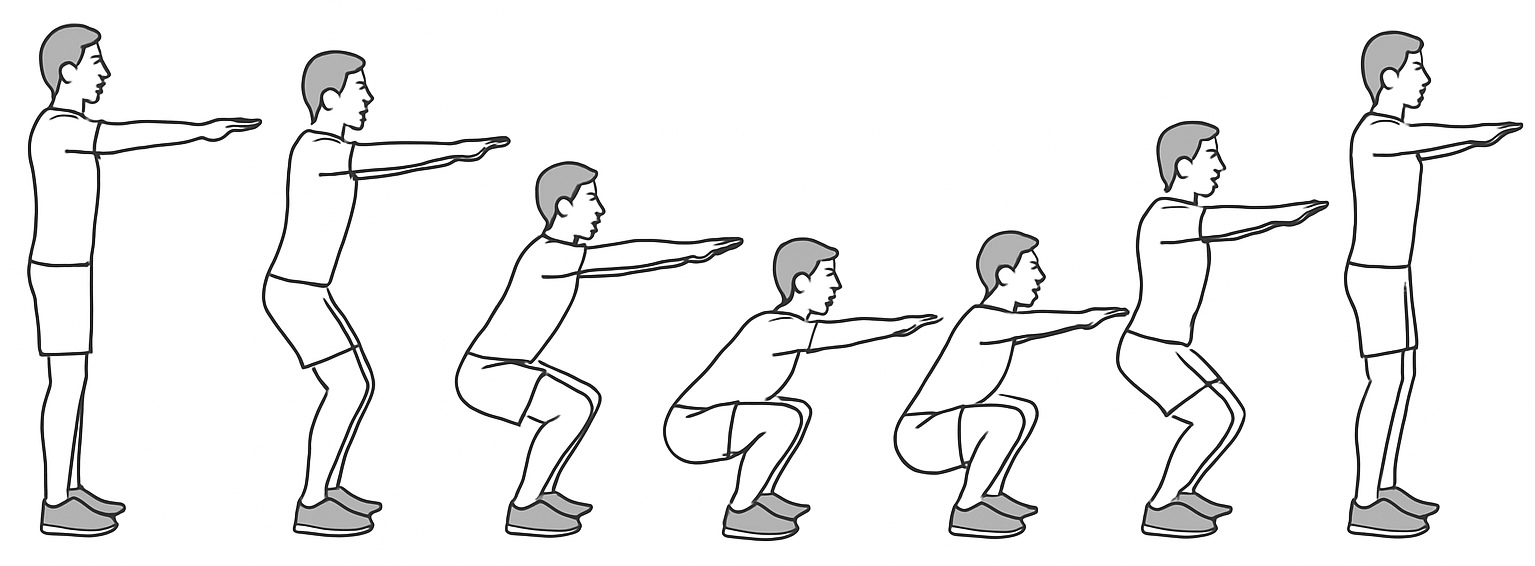
\includegraphics[width=0.75\linewidth]{images/Kniebeuge.jpeg}
\caption{Ablauf einer Kniebeuge, erstellt mit KI-gestützter Bildgenerierung (OpenAI DALL·E 3 via ChatGPT, 2025)}
\label{fig: Kniebeuge}
\end{figure}
\\
\noindent Gestartet wird, wie in Bild 1 zu sehen ist, in aufrechter Haltung. Die Füße stehen schulterbreit und sind leicht nach außen rotiert. Die Arme können zur besseren Balance nach vorne gestreckt werden. Der Rumpf ist angespannt, und die Wirbelsäule befindet sich in einer neutralen Position. \cite{Meinart}

\noindent Wie in Bild 2 dargestellt, wird die Bewegung durch das kontrollierte Zurückschieben des Gesäßes und das Beugen der Knie eingeleitet. Das Körpergewicht bleibt dabei über dem Mittelfuß, während sich der Oberkörper leicht nach vorne neigt. \cite{schoenfeld2010kinematics}

\noindent Während der gesamten Abwärtsbewegung (Bilder 1–3) sollten Hüft-, Knie- und Sprunggelenke gleichzeitig und kontrolliert gebeugt werden. Dabei ist darauf zu achten, dass die Knie nicht über die Fußspitzen hinausragen. \cite{Meinart} Die Kontrolle über die Bewegung wird durch ein bewusst langsames Tempo unterstützt. Studien zeigen, dass eine gute Hüftkontrolle die Belastung auf das Kniegelenk reduziert und die Kraftübertragung optimiert. \cite{schoenfeld2010kinematics} Der Oberkörper sollte möglichst aufrecht bleiben, der Blick nach vorne gerichtet sein, ohne dass der Kopf überstreckt wird. \cite{Meinart}

\noindent Bild 4 zeigt den Tiefpunkt, auch Umkehrpunkt genannt, der Kniebeuge. Je nach Ausführungsvariante ist hier der Kniegelenkswinkel am größten. Die Knie zeigen dabei stabil nach außen. \cite{Meinart}

\noindent Die konzentrische Phase beginnt in Bild 5. Die Aufwärtsbewegung erfolgt durch kraftvolles Drücken aus den Fersen. \cite{schoenfeld2010kinematics} Während der gesamten konzentrischen Phase (Bilder 5–7) sollten Hüft-, Knie- und Sprunggelenke wieder gleichzeitig gestreckt werden. Der Rücken bleibt dabei stabil und gerade, die Füße behalten vollständigen Kontakt zum Boden. \cite{Meinart}

\subsection{Physiologische Grundlagen der Kniebeuge}
\subsubsection{Variationsmöglichkeiten}
\nointent Natürlich gibt es bei der Ausführung einer Kniebeuge verschiedene Variation Möglichkeiten. Zu allem kann eine Kniebeuge mit dem Körpergewicht alleine oder auch mit einem zusätzlichen Gewicht durchgeführt werden. Die Kniebeuge mit der Langhantel ist beispielsweise Bestandteil beim olympischen Gewichtheben. 

\subsubsubsection{Kniebeuge mit Langhantel}
Der grundlegende Bewegungsablauf bei einer Kniebeuge mit Langhantel sollte im Wesentlichen dem einer Körpergewichts Kniebeuge gleichen. Das bedeutet, dass alle Bewegungsmuster, die ohne Zusatzlast bereits sicher beherrscht werden, auch unter Belastung beibehalten werden müssen. Dies ist entscheidend, um Verletzungen vorzubeugen und sicherzustellen, dass durch das zusätzliche Gewicht keine Gelenke oder Muskeln überlastet werden. Besonders wichtig ist dabei eine kontrollierte und stabile Ausführung, bei der die Spannung im gesamten Körper aufrechterhalten wird. \cite{Meinart} Abbildung 2 zeigt drei verschiedene Varianten der Kniebeuge mit einer Langhantel. 
\\
\begin{figure}[ht]\centering
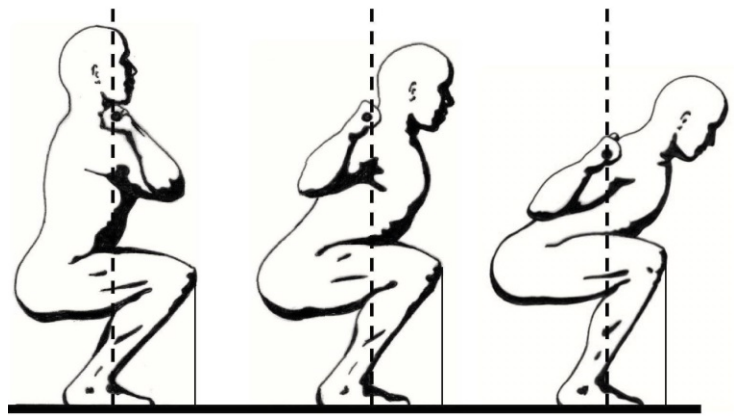
\includegraphics[width=0.75\linewidth]{images/Langhantel_Kniebeuge.png}
\caption{Kniebeugen mit Langhantel, links: Front-Squat, mitte: High Bar, rechts: Low-Bar \cite{Hartmann2014}}
\label{fig: Langhantel}
\end{figure}
\noindent Die Positionierung der Langhantel auf dem Rücken beeinflusst maßgeblich die Körperhaltung während der Kniebeuge. Man unterscheidet hierbei zwischen der „High Bar“- und der „Low Bar“-Technik:
\\
Die „High Bar“-Position ist dadurch gekennzeichnet, dass die Langhantel oberhalb des Schulterdachs auf dem oberen Trapezmuskel abgelegt wird. Diese Variante eignet sich besonders für Anfänger, da sie eine aufrechtere Körperhaltung ermöglicht und den Körperschwerpunkt näher über dem Mittelfuß hält. \cite{Meinart}

\noindent Um die Halswirbelsäule während der Kniebeuge zu schützen, ist es vorteilhaft, eine ausreichende Grundmuskulatur im Nacken- und oberen Rückenbereich aufzubauen. Diese Muskulatur sorgt nicht nur für Stabilität, sondern bietet auch eine natürliche „Polsterung“ für die Langhantel, insbesondere bei der High-Bar-Variante. Ein enger Griff an der Langhantel ist hierbei empfehlenswert. Die Hände sollten so positioniert werden, dass die Unterarme möglichst senkrecht zum Boden stehen. Dies verbessert die Stabilität der Hantel auf dem oberen Rücken und ermöglicht eine präzise Kontrolle während der gesamten Bewegung. \cite{Meinart}
\\
\noindent Im Gegensatz dazu wird die Langhantel beim „Low Bar“-Squat unterhalb des Schulterdach abgelegt. Diese Technik wird häufig bei olympischen Gewichthebern angewendet, da sie eine größere Lastaufnahme ermöglicht. \cite{Meinart}
\noindent Der Griff an der Langhantel kann bei dieser Variante etwas breiter sein, was die Schultergelenke entlastet. Durch die tiefere Ablage der Hantel ergibt sich jedoch eine stärkere Vorlage des Oberkörpers. Diese Vorlage ist notwendig, um den Masseschwerpunkt über dem Mittelfuß zu halten und ein Umfallen nach hinten zu verhindern. durch diese Bewegung Ausführung wird die hintere Muskelkette im Vergleich zur "High Bar" stärker beansprucht. \cite{Meinart}
\\
\noindent Bei der Frontkniebeuge "Front Squat" wird für Fortgeschrittene empfohlen, da diese Ausführung ein höheres Verletzungsrisiko birgt. Die Langhantel wird auf den vorderen Schultern abgelegt, wobei die Hände die Hantel nur stabilisieren und nicht tragen sollen. Der Griff ist leicht breiter als schulterbreit. Die Ellenbogen zeigen nach vorne, die Oberarme bleiben parallel zum Boden, um eine stabile „Front-Rack-Position“ zu gewährleisten. Der Oberkörper sollte möglichst aufrecht bleiben, wobei Gewichtheberschuhe oder erhöhte Fersen dabei unterstützen. Während des gesamten Bewegungsablaufs bleiben Hüfte, Knie und Sprunggelenke synchron in Bewegung, um die Balance zu halten und den Masseschwerpunkt über dem Mittelfuß zu stabilisieren. Alternativ kann die Langhantel in der „Bodybuilding-Variante“ mit überkreuzten Armen gehalten werden, was die Mobilitätsanforderungen reduziert. Die Frontkniebeuge eignet sich ideal zur Kräftigung der vorderen Oberschenkelmuskulatur. \cite{Meinart}

\subsubsection{erreichte Kniegelenkswinkel während einer Kniebeuge}
\noindent Die optimale Tiefe einer Kniebeuge hängt von der individuellen Zielsetzung ab. 
\noindent Für den Muskelaufbau sind tiefe Kniebeugen mit einem Kniewinkel von 40–70° vorteilhaft.\cite{Hartmann2014} Bei korrekter Ausführung und in Abwesenheit von Kniepathologien sind tiefe Kniebeugen nicht schädlich für das Kniegelenk.\cite{Hartmann2014} 

\noindent Bei einer halben Kniebuege spricht man, von einem Kniewinkel von ca. 80-100°. \cite{Hartmann2014} Diese Art der Kniebeuge belastet das Knie häufig mehr als bei einer tiefen Kniebeuge. Dies liegt an den auftretenden Bremskräften kurz vor dem Umkehrpunkt der Bewegung. Im Gegensatz dazu können bei tiefen Kniebeugen die Lasten um 30–50\% geringer sein als bei halben Kniebeugen.\cite{Tiefe}

\noindent Die Viertelkniebeuge entspricht einer geringen Beugung des Knies, im Bereich von ca. 110-140°. \cite{Hartmann2014} In diesem Bereich gibt es wenig Muskelaufbau. Jedoch können hier die größten Lasten gehoben werden. \cite{Tiefe}

\noindent Nach einer Knieverletzung, insbesondere nach einer Kreuzbandverletzung, sollte die Tiefe der Kniebeuge jedoch auf 50–60\% der normalen Bewegung begrenzt werden, um das Gelenk zu entlasten und eine Überlastung der Strukturen zu vermeiden. \cite{Tiefe}

\subsubsection{Allgemein beanspruchte Muskulatur bei einer Kniebeuge}
\noindent Bei einer Kniebeuge sind viele Muskeln beteiligt. Je nach Ausführung variiert die Beanspruchung der Muskulatur. Im folgenden werden die wichtigsten Muskeln in der Kniebeuge aufgelistet. 

\noindent \textbf{Die Wadenmuskulatur} setzt sich aus dem \textbf{M. soleus} und dem \textbf{M. gastrocnemius} zusammen, die während der Kniebeuge unterschiedliche Funktionen erfüllen. Der M. soleus wird vor allem bei einem größeren Kniewinkel aktiviert und spielt in der Aufwärtsbewegung eine zentrale Rolle, da er maßgeblich zur Plantarflexion beiträgt – also zur Bewegung des Fußes im oberen Sprunggelenk in Richtung der Fußsohle. Im Gegensatz dazu unterstützt der M. gastrocnemius sowohl die Plantarflexion als auch die Beugung des Knies, wobei seine Aktivität insbesondere in den ersten 15 Grad der Kniebeuge am höchsten ist. \cite{Meinart}

\noindent \textbf{Der M.gluteus maximus}, der große Gesäßmuskel, ist bei der Kniebeuge sowohl für die Bewegung als auch für die Stabilisierung verantwortlich. Während der Abwärtsbewegung arbeitet er kontrollierend (extentrisch), beim Aufrichten sorgt er für die notwendige Kraftentfaltung (konzentrisch). Er unterstützt die Hüftstreckung und hilft, das Knie zu stabilisieren. Besonders stark beansprucht werden die unteren Muskelanteile, vor allem im tiefsten Punkt der Kniebeuge. \cite{Meinart}

\noindent \textbf{Die ischiocrurale Muskulatur (Hamstring)}, die hintere Oberschenkelmuskulatur, ist während der Kniebeuge nur gering aktiv. Besonders im oberen Bewegungsabschnitt (bei Teilkniebeugen) zeigt sie etwas mehr Aktivität, während die tiefe Kniebeuge kaum zusätzliche Reize setzt. Da der Beinbeuger sowohl für die Beugung des Knies als auch für die Streckung der Hüfte zuständig ist und beide Gelenke während der Kniebeuge gleichzeitig beugen, verändert sich seine Länge kaum. \cite{Meinart}

\noindent \textbf{Der Musculus adductor magnus} ist ein großer, dreieckiger Muskel an der Innenseite des Oberschenkels, der eine wesentliche Rolle bei der Hüftstreckung während der Kniebeuge spielt. Aufgrund seines Ursprungs am Sitzbein (Tuber ischiadicum) wird er oft als “vierter Beinbeuger” bezeichnet, obwohl er nicht am Kniegelenk ansetzt und somit ausschließlich auf die Hüfte wirkt. \cite{Meinart}

\noindent \textbf{Der Musculus quadriceps femoris} besteht aus vier Muskeln. Der Musculus rectus femoris verläuft über Hüft- und Kniegelenk und ermöglicht besonders die Hüftbeugung aber auch Kniestreckung. Der Musculus vastus lateralis, intermedius und medialis liegen am Oberschenkelknochen und sind primär für die Kniestreckung verantwortlich. Für die Kniestabilität ist besonders der Musculus vastos bedeutend. \cite{Meinart}
\\
\noindent In der Abbildung 3 sind die genannten Muskeln und noch weitere Muskeln der Beine abgebildet. 
\\
\begin{figure}[ht]\centering
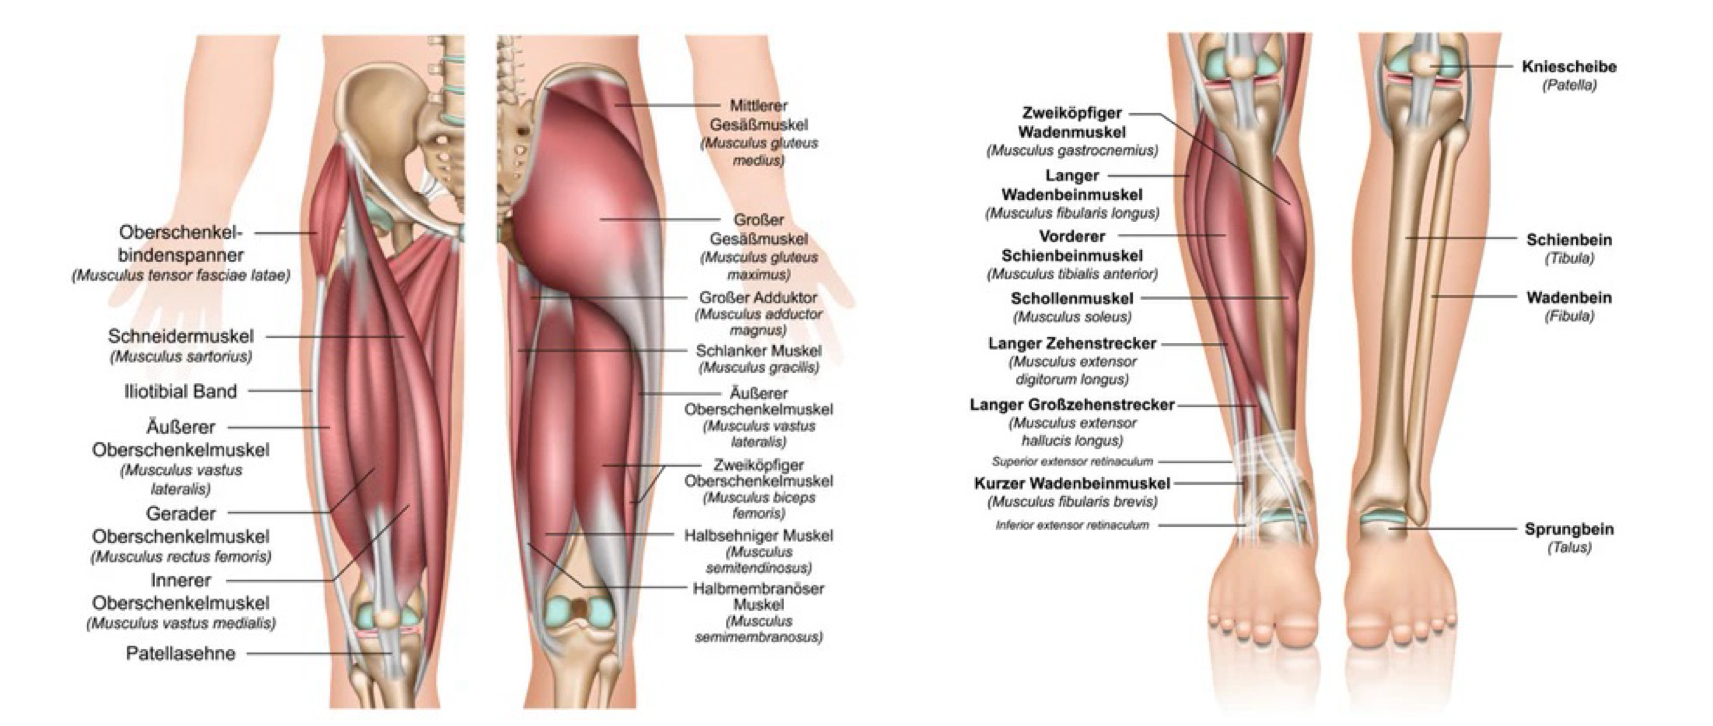
\includegraphics[width=1\linewidth]{images/Muskeln.jpeg}
\caption{Beinmuskulatur (links Oberschenkel, rechts Unterschenkel)\cite{GorillaSports_Beintraining}}
\label{fig: Beinkuskulatur}
\end{figure}
\\
\\
\\
\subsubsection{Vergleich verschiedener Kniebeugen-Tiefen und ihre muskuläre Wirkung}
Die Tiefe einer Kniebeuge hat einen erheblichen Einfluss darauf, welche Muskelgruppen besonders beansprucht werden. Je nach Bewegungsausmaß lassen sich drei wesentliche Varianten unterscheiden: die tiefe Kniebeuge (auch „Ass to Grass“), die halbe Kniebeuge (Parallel Squat) sowie die Viertel-Kniebeuge (Quarter Squat). Jede dieser Varianten aktiviert die Muskulatur in unterschiedlichem Ausmaß.\cite{Meinart}
\\
\\
\noindent \textbf{Die tiefe Kniebeuge} beschreibt eine Ausführung, bei der die Hüfte unterhalb der Kniehöhe absinkt. In dieser Variante werden insbesondere der \textit{Gluteus maximus}, die \textit{Adduktoren} sowie die \textit{Vastus-Gruppe} des Quadrizeps maximal beansprucht. Die große Bewegungsamplitude sorgt für eine starke Dehnung und Aktivierung dieser Muskelgruppen. Vor allem die unteren Fasern des Gluteus maximus sowie der M. adductor magnus arbeiten hier besonders intensiv. Diese Variante ist besonders effektiv für Muskelaufbau, Mobilität und funktionelle Kraft, da sie viele alltagsrelevante Bewegungen abbildet und durch die tiefe Position eine verbesserte Beweglichkeit fördert. \cite{Meinart}
\\
\\
\noindent \textbf{Die halbe Kniebeuge}, bei der die Oberschenkel parallel zum Boden verlaufen, aktiviert primär den Quadrizeps und in geringerem Maße den Gluteus. Die Adduktoren sind in dieser Bewegung nur moderat involviert. Diese Variante ist gelenkschonender als die tiefe Kniebeuge und wird häufig im Kraftdreikampf verwendet, da sie eine gute Balance zwischen Kraftentwicklung und technischer Sicherheit bietet. Durch den reduzierten Bewegungsweg können oft höhere Lasten als bei der tiefen Variante bewegt werden, ohne dabei das Risiko für Überlastung zu erhöhen. \cite{Meinart}
\\
\\
\noindent \textbf{Die Viertel-Kniebeuge} zeichnet sich durch eine sehr geringe Knieflexion aus. Diese Bewegung aktiviert den Beinbeuger (die ischiocrurale Muskulatur) in höherem Maße als die tiefere Variante, da in diesem Bereich die EMG-Aktivität der Hamstrings am stärksten ist. Der Quadrizeps wird hingegen nur minimal beansprucht. Aufgrund der kurzen Bewegungsamplitude eignet sich diese Form insbesondere für Schnellkrafttraining oder sportartspezifische Reize, etwa in Sprungsportarten. Auch im Rehabilitationsbereich kann sie gezielt eingesetzt werden, um Teilbewegungen zu trainieren, ohne die Gelenke zu stark zu belasten. \cite{Meinart}
\\
\\
Zusammenfassend lässt sich sagen, dass die Tiefe der Kniebeuge nicht nur die Belastung der beteiligten Gelenke, sondern vor allem auch die Aktivierung bestimmter Muskelgruppen beeinflusst. Für den gezielten Aufbau von Gesäß- und Adduktorenmuskulatur eignet sich die tiefe Kniebeuge am besten. Wer dagegen den Fokus auf reine Kraftentwicklung oder Schnelligkeit legt, kann von der halben oder gar viertel Kniebeuge profitieren. Die Auswahl der richtigen Variante sollte stets vom Trainingsziel, dem Leistungsstand und der individuellen Anatomie abhängig gemacht werden. \cite{Meinart}

\subsection{Wissenschaftliche Publikation}
\noindent Die präzise Erfassung des Kniegelenkswinkels ist ein zentrales Thema in der orthopädischen Diagnostik, Rehabilitation sowie in sportwissenschaftlichen und medizintechnischen Anwendungen. In den letzten Jahren hat die Forschung erhebliche Fortschritte gemacht. 

\noindent In der Studie „Repeatability of measuring knee flexion angles with wearable inertial sensors“ wurde die Reproduzierbarkeit der Kniewinkelmessung mithilfe tragbarer Inertialsensoren (IMUs) untersucht. Zu diesem Zweck kam ein roboterbetriebenes Beinmodell zum Einsatz, das standardisierte Flexionsbewegungen ausführte, welche Bewegungen wie Kniebeugen simulierten. Zur Erfassung der Bewegungsdaten wurden je ein IMU am Oberschenkel und am Unterschenkel positioniert, jeweils entweder posterior (rückseitig) oder lateral (seitlich). Als Referenzsysteme dienten ein Elektrogoniometer sowie ein optisches 3D-Motion-Capture-System. Die Ergebnisse zeigten, dass beide IMU-Positionierungen eine hohe Wiederholgenauigkeit aufwiesen. Die maximalen Flexionswinkel wurden mit durchschnittlichen Abweichungen von ±1,1° (lateral) bzw. ±2,4° (posterior) im Vergleich zur Referenz gemessen. Während die Bewegungsgeschwindigkeit nur einen geringen Einfluss auf die Messgenauigkeit hatte, führten Positionsveränderungen der Sensoren zu deutlich größeren Messabweichungen. Das lateral angebrachte IMU-Setup erzielte die besten Resultate, was vermutlich auf eine höhere Stabilität und bessere Reproduzierbarkeit der Platzierung zurückzuführen ist. Die Auswertung der Sensordaten erfolgte mittels eines eigens entwickelten MATLAB-Programms zur Berechnung des Kniewinkels. Insgesamt belegt die Studie, dass IMUs in Kombination mit einer softwaregestützten Auswertung eine kosteneffiziente, portable und zugleich zuverlässige Methode zur Messung des Kniewinkels darstellen. Dies gilt insbesondere für dynamische Bewegungsanalysen, wie sie beispielsweise bei Kniebeugen auftreten. Die Autoren schließen daraus, dass IMUs eine valide Alternative zu klassischen Goniometern oder komplexen Motion-Capture-Systemen darstellen. \cite{Fennema2019}
\\
\noindent Ein weiterer Ansatzpunkt ist die Videoanalyse. Sowohl 2D- als auch 3D-basierte Verfahren werden eingesetzt, um Gelenkwinkel nichtinvasiv zu erfassen. Während 3D-Systeme sehr präzise, aber kostenintensiv sind, zeigen aktuelle Studien eine zunehmende Validität auch von 2D-Systemen. 
\\
\noindent In der Studie von Chida et al. (2024) wurde die Validität der zweidimensionalen (2D) Videoanalyse zur Erfassung der Gelenkwinkel der unteren Extremität während eines Fecht-Ausfallschritts untersucht. Ziel war es, die 2D-Analyse als potenziell kostengünstige und praxistaugliche Alternative zur dreidimensionalen (3D) Bewegungsanalyse zu evaluieren. Insgesamt 22 männliche Fechter führten standardisierte Lunge-Bewegungen aus, die gleichzeitig mit einem 3D-Motion-Capture-System (Qualisys) und zwei Digitalkameras aufgezeichnet wurden. Die Analysen konzentrierten sich auf die Zeitpunkte des Abstoßens (heel-off) und des Aufsetzens (heel-strike) des vorderen Beins. Die Ergebnisse zeigten eine sehr hohe Übereinstimmung der Kniewinkel zwischen 2D- und 3D-Analyse bei Abweichungen von maximal ±4,3°, was auf eine hohe Messgenauigkeit der 2D-Methode in der Sagittalebene hinweist. Dagegen zeigten die Messwerte für das Hüft- und Sprunggelenk größere Abweichungen, insbesondere bei der Sprunggelenksanalyse mit einer Überschätzung von bis zu 21,3° durch die 2D-Methode. Die Autoren schlussfolgern, dass die 2D-Videoanalyse eine valide Methode zur Messung des Kniewinkels bei Bewegungen mit geringen Rotationsanteilen darstellen kann. Sie eignet sich besonders für sportpraktische Anwendungen, bei denen keine aufwendige Messtechnik verfügbar ist. \cite{videoanalysis2024}
\nointent Es gibt beispielsweise Anwendungen wie Kniovea, die frei zugänglich sind und zur Winkelanalyse eingesetzt werden. \cite{Kniovea}

\section{Ziel der Arbeit}
\noindent Die korrekte Ausführung einer Kniebeuge ist entscheidend, um Verletzungen zu vermeiden und bestimmte Muskelgruppen gezielt zu trainieren. Zur Analyse des während der Bewegung erreichten Kniegelenkswinkels stehen unterschiedliche Verfahren zur Verfügung.
\\
\noindent Konventionelle Methoden wie Videoanalysen (z.\,B. mit \textit{Kinovea}) bieten zwar wertvolle visuelle Informationen, sind jedoch aufwendig, häufig subjektiv in der Auswertung und erfordern entweder manuelle Winkelmessung oder kostenintensive Softwarelösungen wie \textit{Contemplas}.
\\
\noindent Die Kombination der \textit{Phyphox}-App mit einer eigens entwickelten grafischen Benutzeroberfläche (GUI) in \textit{MATLAB} ermöglicht eine moderne, praxisnahe und zugängliche Methode zur Erfassung und Analyse des Kniegelenkswinkels. Im Gegensatz zu klassischen Messsystemen wie Goniometern oder komplexen Bewegungslaboren bietet diese Methode eine mobile, kostengünstige und benutzerfreundliche Lösung basierend auf handelsüblichen Smartphones. Die integrierten Sensoren liefern eine ausreichende Genauigkeit für Bewegungsanalysen, insbesondere bei Bewegungsmustern wie der Kniebeuge.
\\
\noindent Ein zentrales Ziel dieser Arbeit ist es, durch die Entwicklung einer MATLAB-GUI eine automatisierte und visuell unterstützte Auswertung der Messdaten zu ermöglichen. Die GUI erlaubt es, Winkelverläufe darzustellen und automatisiert anhand der gewählten Kniebeugen-Variante zu bewerten. Damit eignet sich das System sowohl für den sportwissenschaftlichen Einsatz als auch für Privatpersonen, die ihre Ausführung analysieren und verbessern möchten.

\subsection{Vorteile der sensorbasierten Auswertung}
\noindent Die hier vorgestellte sensorbasierte Methode mit der \textit{Phyphox}-App zeigt einige Vorteile:
\begin{itemize}
  \item \textbf{Objektiv:} Die automatische Analyse minimiert subjektive Einflüsse.
  \item \textbf{Zeitsparend:} Die direkte Auswertung der CSV-Daten macht eine manuelle Nachbearbeitung überflüssig.
  \item \textbf{Zugänglich:} Sie basiert auf frei verfügbarer Software und handelsüblichen Smartphones.
  \item \textbf{Flexibl:} Schwellenwerte für die Beurteilung der Kniebeugen sind individuell anpassbar – z.\,B. für Reha- oder Trainingszwecke.
\end{itemize}

\subsection{Funktionsweise der Auswertung}

\noindent Die Auswertung einer Kniebeuge mittels \textit{Phyphox} erfolgt über zwei GUIs:

\begin{itemize}
  \item \textbf{GUI 1 – Kalibrierung:} Diese Oberfläche dient der Kalibrierung der Smartphone-Sensoren, um eine zuverlässige Erfassung des tatsächlichen Kniegelenkswinkels zu gewährleisten. 
  \item \textbf{GUI 2 – Auswertung:} Diese GUI dient der eigentlichen Analyse. Nach Auswahl der gewünschten Kniebeugen-Variante (z.\,B. tief, halb, viertel) wird ein entsprechender Informationstext angezeigt. Gleichzeitig werden automatisch passende Schwellenwerte für die spätere Auswertung gesetzt.
\end{itemize}

\noindent Im Anschluss lädt die Nutzerin bzw. der Nutzer zwei CSV-Dateien, die mithilfe der \textit{Phyphox}-App erstellt wurden. Die Software analysiert daraufhin, wie viele Kniebeugen innerhalb, oberhalb oder unterhalb der definierten Schwellenwerte lagen. 
\\
\noindent Das Ergebnis wird zweifach dargestellt:
\begin{itemize}
    \item \textbf{Visuell:} Im Diagramm zeigt eine blaue Linie den zeitlichen Verlauf des Kniegelenkswinkels. Die gesetzten Schwellenwerte werden durch rot-gestichelte Linien dargestellt. Die gemessenen Winkelwerte der Kniebeugen werden farblich markiert: grün (innerhalb), rot (außerhalb).
    \item \textbf{Textlich:} Ein Auswertungsfeld fasst die Ergebnisse zusammen mit Angabe der Gesamtzahl der Kniebeugen sowie deren Einordnung (innerhalb, oberhalb, unterhalb der Schwellen), dazu wird noch eine Rückmeldung zur Durchschnittlichen Tiefe in Grad angezeigt. 
\end{itemize}

\subsection{Anwendungsbereich}

\noindent Da zu Beginn der Analyse eine bevorzugte Kniebeugen-Variante gewählt werden kann, eignet sich die Anwendung für verschiedene Zielgruppen und Einsatzszenarien. Durch die Kombination aus objektiver Sensorik und flexibler Software lässt sich das System einfach individualisieren.
\\
\noindent
Im folgenden Kapitel~5 wird ein praktischer Versuch mit mehreren Probanden beschrieben, um die Funktionalität und Aussagekraft der App zu überprüfen. Die Versuchsdurchführung ist dabei so gestaltet, dass sie auch von Privatpersonen eigenständig nachvollzogen werden kann.
\section{Technischer Hintergrund}
\subsection{ Beschleunigungssensoren}
\noindent In diesem Versuch wurden zu einem ein IPhone 12 mini und ein IPhone 11 verwendet. 
Für die Messung wurde ein \textit{iPhone 12 mini} (Modell: iPhone13,1) verwendet. Das Gerät stammt vom Hersteller Apple, die verwendete Stichprobengröße basiert auf 292 Geräten, wobei es sich um eine Gerätevariante handelt. Das integrierte \textbf{Beschleunigungssensor-Modul (Accelerometer)} des iPhones ist verfügbar und weist folgende Eigenschaften auf \cite{phyphoxSensorDB}:
\begin{itemize}
  \item \textbf{Abtastrate:} 100{,}0\,Hz
  \item \textbf{Durchschnittlicher Beschleunigungswert (im Ruhezustand):} 9{,}820\,m/s\textsuperscript{2}
  \item \textbf{Standardabweichung:} 0{,}018\,m/s\textsuperscript{2}
\end{itemize}
\noindent Diese Werte deuten auf eine hohe Genauigkeit und Stabilität des Sensors hin, was ihn für Bewegungsanalysen – wie beispielsweise die Bestimmung des Kniewinkels bei Kniebeugen – geeignet macht.
\\
\\
Zusätzlich kam ein \textit{iPhone 11} (Modell: iPhone12,1) zum Einsatz. Auch dieses Gerät stammt vom Hersteller Apple. Die zugrunde liegende Stichprobengröße umfasst 696 Geräte, wobei ebenfalls nur eine Gerätevariante berücksichtigt wurde. Der integrierte \textbf{Beschleunigungssensor (Accelerometer)} des iPhone 11 besitzt folgende Eigenschaften \cite{phyphoxSensorDB}:
\begin{itemize}
  \item \textbf{Abtastrate:} 100{,}0\,Hz
  \item \textbf{Durchschnittlicher Beschleunigungswert (im Ruhezustand):} 9{,}840\,m/s\textsuperscript{2}
  \item \textbf{Standardabweichung:} 0{,}015\,m/s\textsuperscript{2}
\end{itemize} 
\noindent Diese technischen Daten belegen ebenfalls eine hohe Genauigkeit und geringe Streuung der Sensordaten, was die Eignung des Geräts für präzise Bewegungsanalysen wie Kniebeugenmessungen bestätigt. 

\subsection{Phyphox-App}
Damit die Bewertung einer Kniebeuge von jeder Person durchgeführt werden kann, wird die kostenlose App \textit{Phyphox} verwendet. \textit{Phyphox} ist eine Marke der RWTH Aachen, eingetragen in Deutschland, der EU, den USA und anderen Ländern. \noindent Die App \textit{Phyphox} kann kostenlos auf Smartphones installiert werden \cite{phyphoxDownload}. 
Für iOS-Geräte ist sie im \href{https://apps.apple.com/us/app/phyphox/id1127319693?l=de&ls=1}{App Store} erhältlich, 
für Android-Geräte im \href{https://play.google.com/store/apps/details?id=de.rwth_aachen.phyphox}{Google Play Store}.
\\
\noindent Die App umfasst verschiedene Funktionen, zu einem können die Sensoren des Smartphones verwendet werden um zu experimentieren, es ist ein Daten Export in verschiedenen Formaten möglich, es ist eine Fernsteuerung zu einem Web-Browser möglich, und es können eigene Experimente erstellt werden. In der App stehen einem viele Möglichkeiten zur Verfügung. Es wird unterschieden in Sensoren, Akustik, Alltag, Mechanik, Werkzeuge und Zeitmessung. In der Abbildung 4 sind die einzelnen Auswahlmöglichkeiten der Kategorien ersichtlich. \cite{Phyphox}
\begin{figure}[ht]\centering
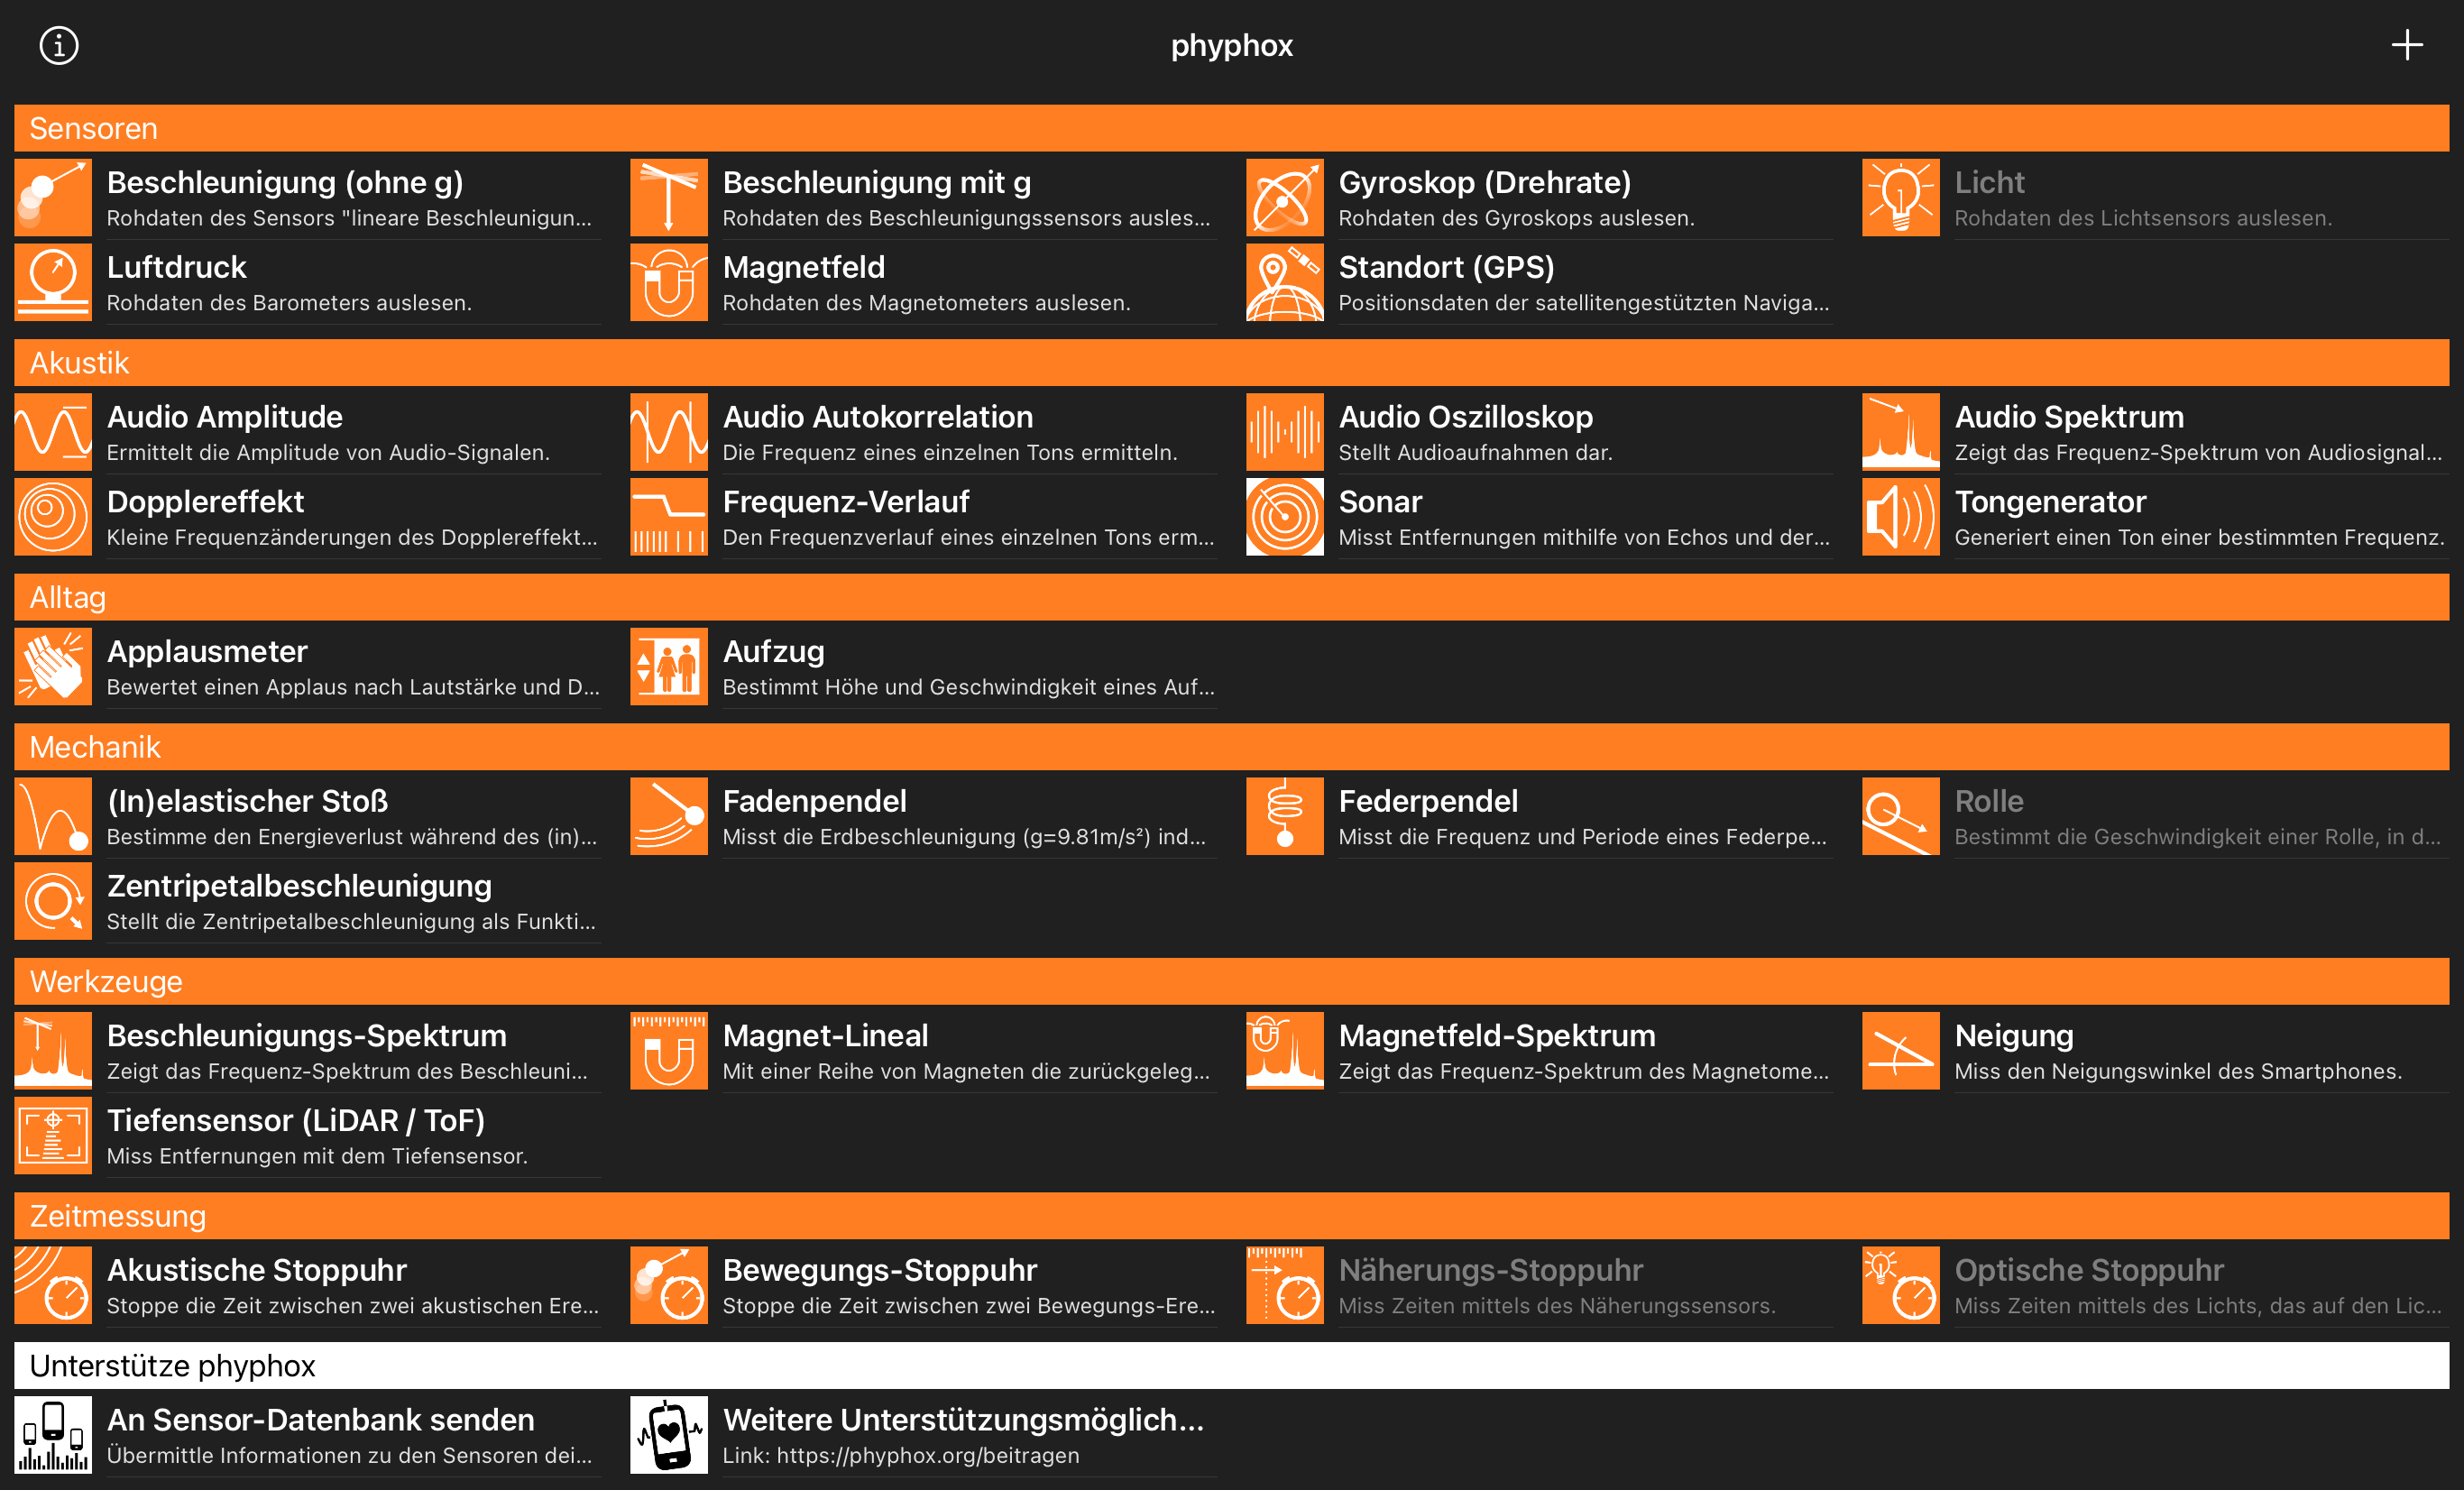
\includegraphics[width=\linewidth]{images/Phyphox.jpeg}
\caption{Anwenderoberfläche Phyphox \cite{Phyphox}}
\label{fig:Anwenderoberfläche Phyphox}
\end{figure}

\noindent Für die Aufnahme der Beschleunigungsdaten, die zur Auswertung der Kniebeuge benötigt werden, wird in der Kategorie Sensoren der Tab Beschleunigung mit G ausgewählt. Dadurch können die Daten des im Smartphone integrierten Beschleunigungssensors erfasst werden. Dabei wird die Gravitationskraft berücksichtigt, sodass konstant eine Beschleunigung auch ohne Bewegung von 9,81 m/s² angezeigt wird. \cite{Phyphox} Jenachdem in welcher Lage sich das Smartphone befindet, werden die Beschleunigung unterschiedlich auf die Achsen verteilt.
\\
\noindent Die Abbildung 5 veranschaulicht den Ablauf der Datenerhebung und des Exports mit der Smartphone-Applikation \textit{Phyphox} am Beispiel des Sensors „Beschleunigung mit g“. Nach dem Öffnen der App wird zunächst das entsprechende Sensor-Modul ausgewählt, das die dreidimensionale Beschleunigung unter Berücksichtigung der Gravitationskomponente erfasst (erstes Bild von links). Mit Betätigung der Aufnahmetaste wird die Messung gestartet (zweites Bild), wobei die Beschleunigungswerte in den Raumrichtungen x, y und z über die Zeit hinweg aufgezeichnet und grafisch dargestellt werden. Nach Beendigung der Aufnahme (drittes Bild) kann das Aktionsmenü (Symbol mit drei Punkten) geöffnet werden (viertes Bild). Über die Option „Daten exportieren“ (fünftes Bild) öffnet sich das Dialogfenster (sechses Bild) um das gewünschte Dateiformat für den Export auszuwählen. Für die Weiterverarbeitung der Messdaten in Programmen wie MATLAB oder Excel empfiehlt sich die Auswahl des CSV-Formats mit Komma als Dezimaltrennzeichen (CSV (Comma, decimal point)). Der Export der aufgezeichneten Daten erfolgt anschließend durch Auswahl des Buttons „Daten exportieren“.
\begin{figure}[ht]\centering
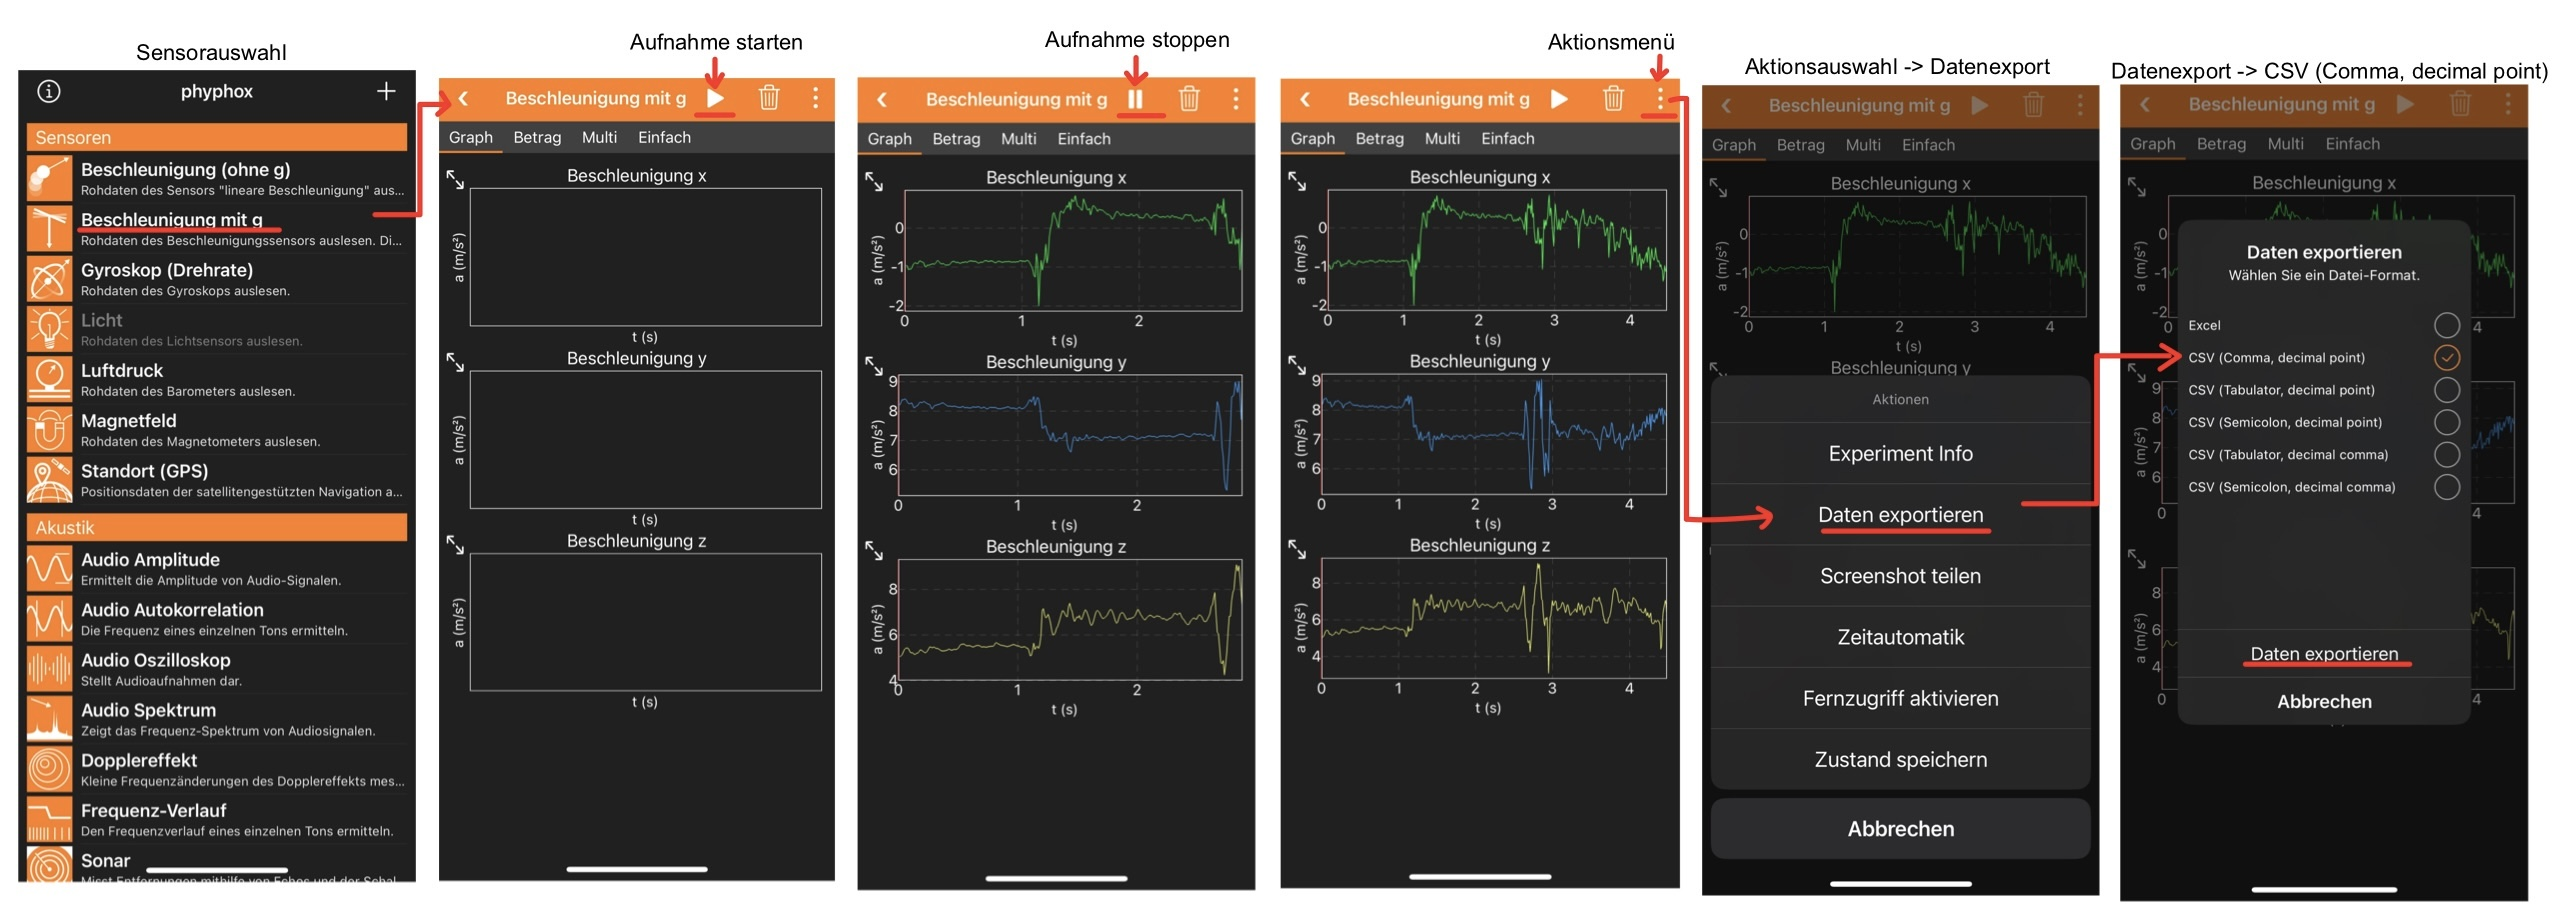
\includegraphics[width=\linewidth]{images/Bedienung.jpeg}
\caption{Bedienung Phyphox am Beispiel Beschleunigung mit g\cite{Phyphox}}
\label{fig:Anwenderoberfläche Phyphox}
\end{figure}
\subsection{Experiment zur Darstellung der App}
\noindent Im folgenden wird ein kleines Experiment untersucht, welches die Messung der Erdbeschleunigung mit einem Smartphone darstellt. Aus der Kategorie Sensoren wird der Tab Beschleunigung mit g ausgewählt. Nach dem Start über den Play-Button oben rechts, befindet sich das Smartphone zunächst flach auf dem Tisch. Danach wird es auf die Längskante gekippt und schließlich hochkant aufgestellt. Während des gesamten Versuchs erfasst der Sensor die Beschleunigung in den verschiedenen Positionen.
\\
\noindent In der Abbildung 6 sind die Messdaten des Experiments dargestellt. Die grüne Kurve zeigt die Beschleunigung entlang der X-Achse, die blaue Kurve die Beschleunigung entlang der Y-Achse, die gelbe Kurve die Beschleunigung entlang der Z-Achse und die weiße Kurve die absolute Beschleunigung. Die Werte unter dem Graphen geben die gemessene Beschleunigung zum Zeitpunkt des Stopps des Experiments an. In diesem Fall wurde die Option “Multi” ausgewählt, wodurch alle Kurven in einem gemeinsamen Diagramm dargestellt werden. Alternativ besteht die Möglichkeit, die einzelnen Achsen in separaten Diagrammen darzustellen. Diese Funktion steht unter der Option “Graph” zur Verfügung. 
\noindent Um die Achsenzuordnung genauer nachvollziehen zu können, ist diese in Abbildung 7 dargestellt. Die Abbildung 7 zeigt die Orientierung der X-, Y- und Z-Achse relativ zum Smartphone, wie sie in der verwendeten App zur Beschleunigungsmessung Phyphox verwendet wird.
\\
\begin{figure}[ht]\centering
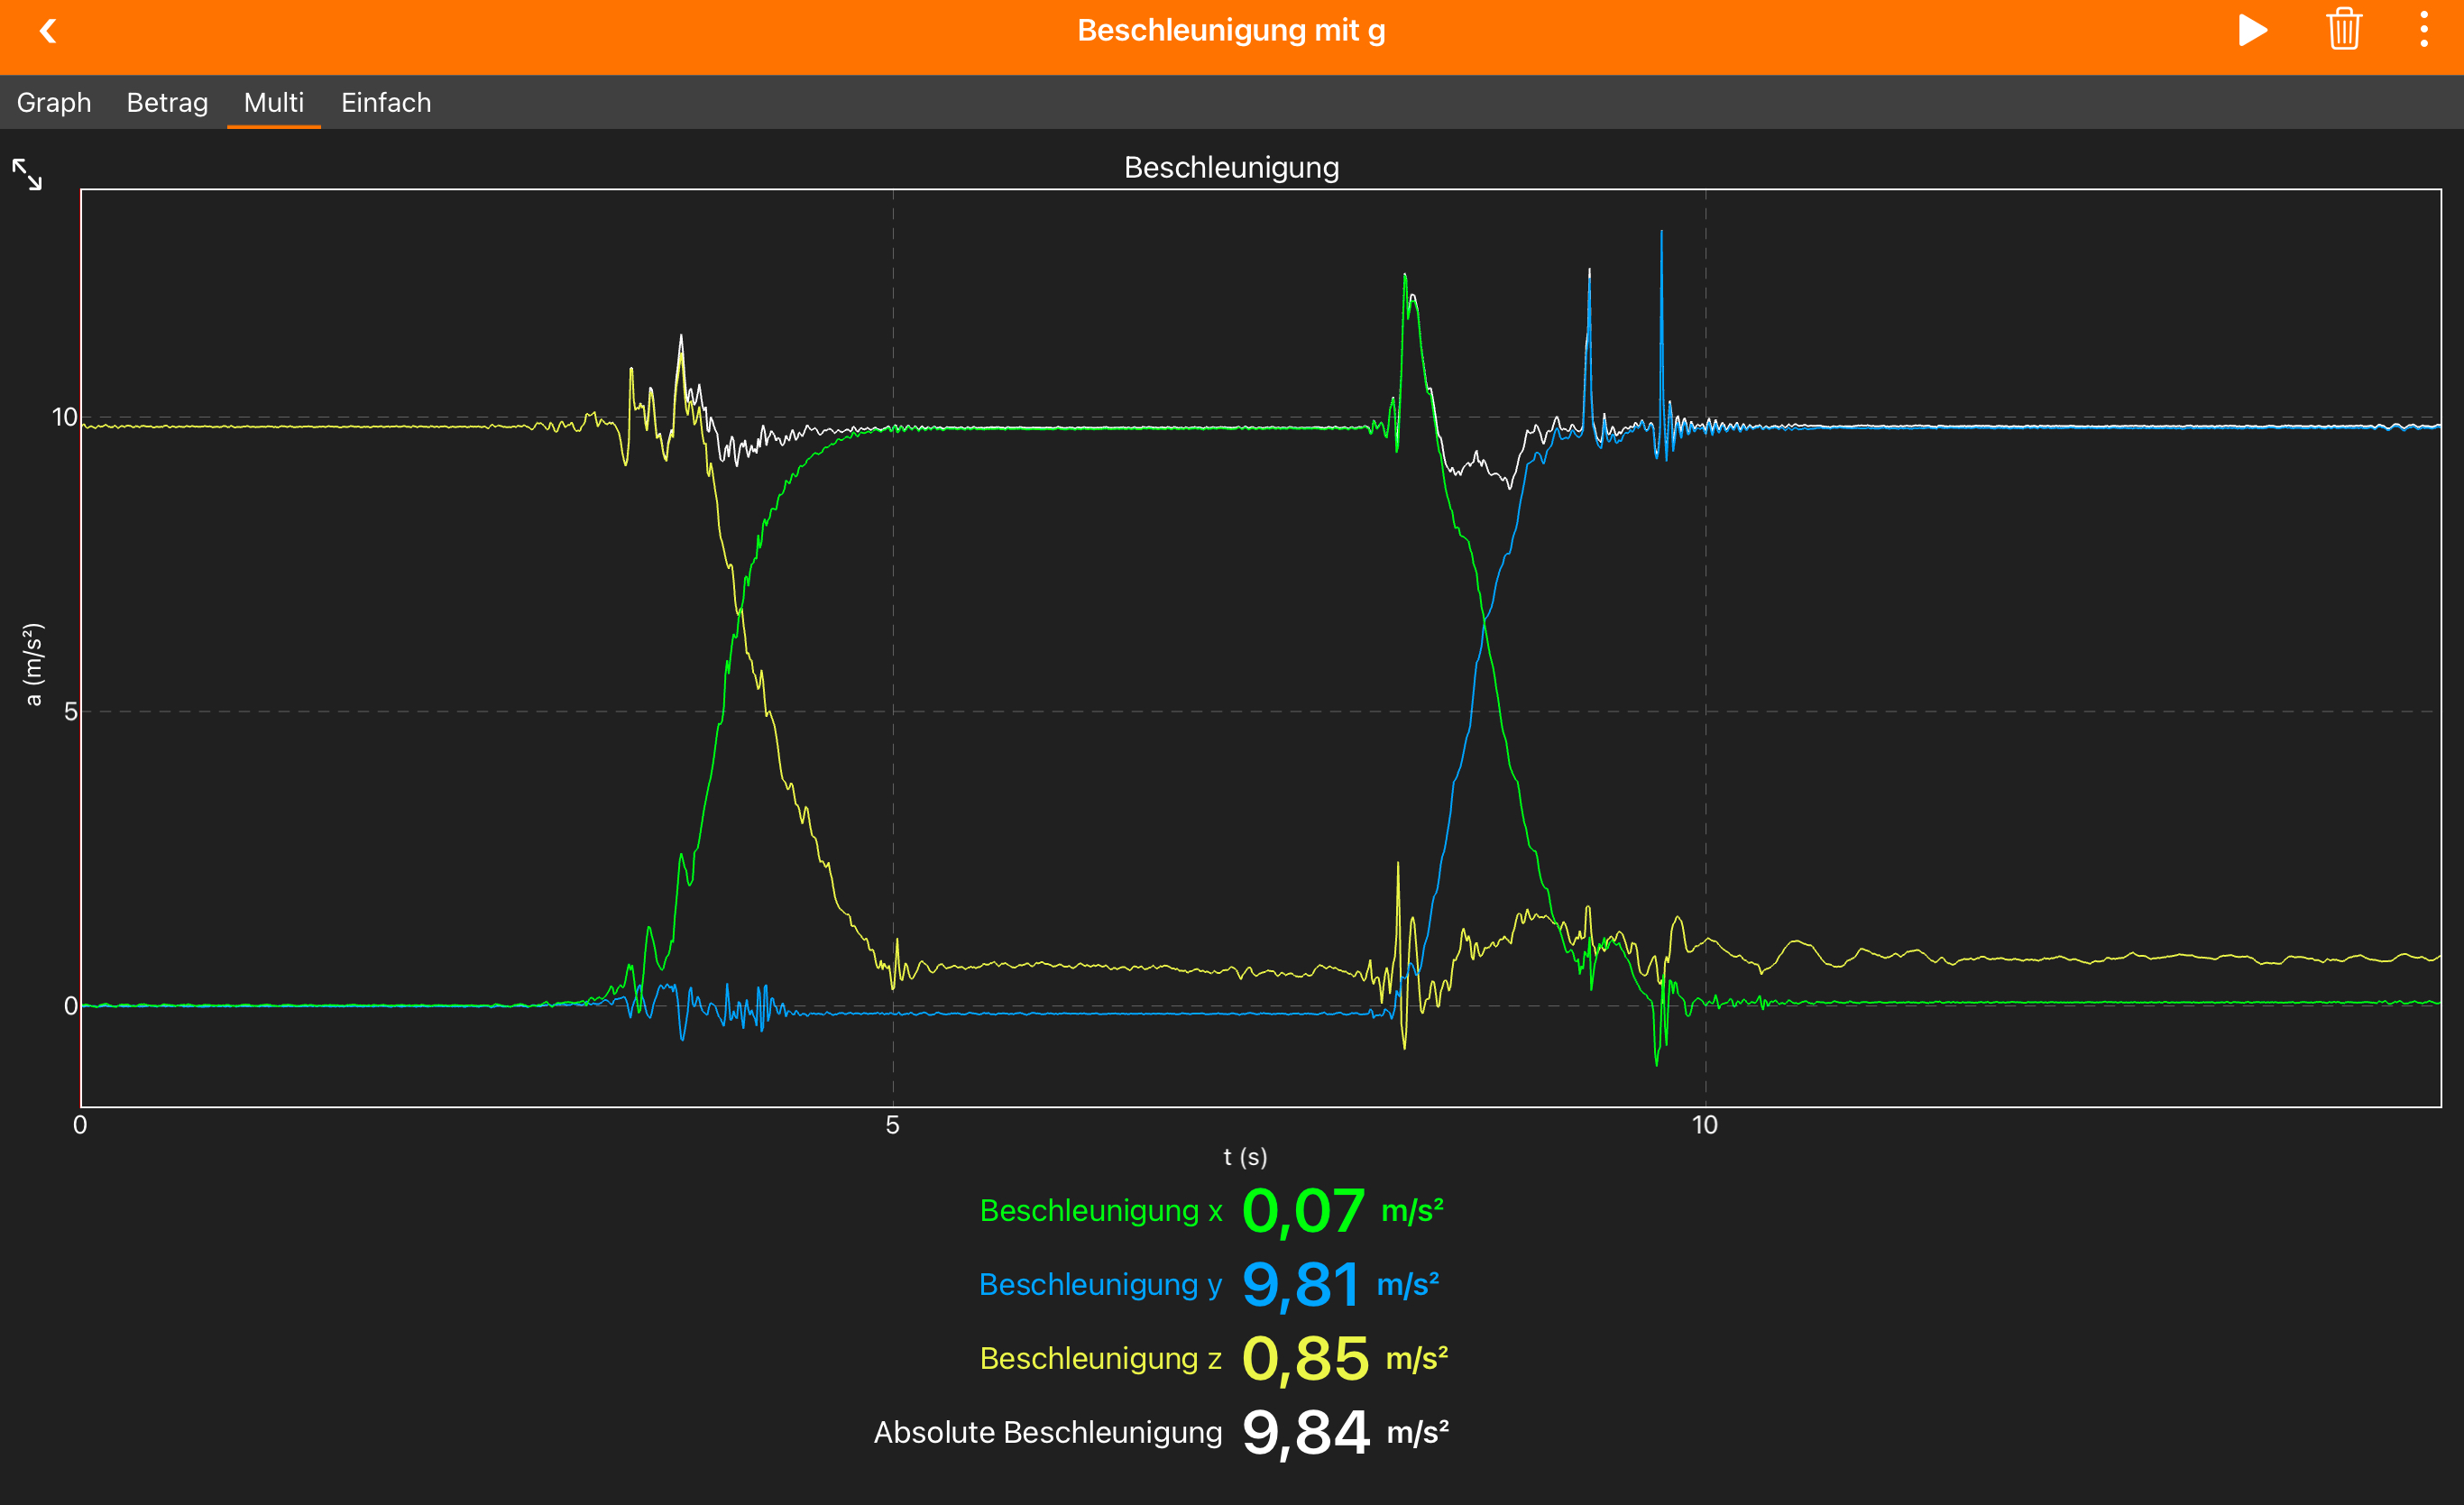
\includegraphics[width=0.75\linewidth]{images/Beschleunigung.jpeg}
\caption{Versuch Beschleunigungsdaten \cite{Phyphox}}
\label{fig:Versuch Beschleunigungsdaten}
\end{figure}
\begin{figure}[ht]\centering
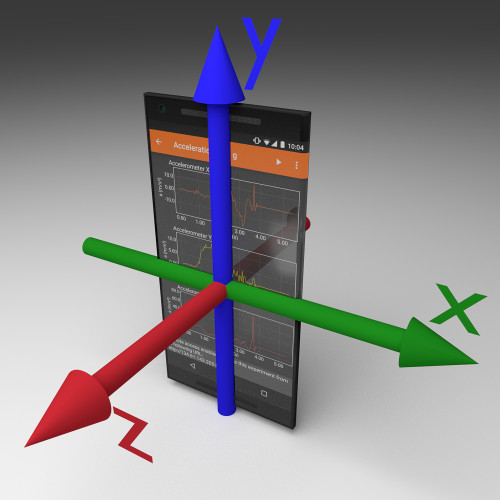
\includegraphics[width=0.35\linewidth]{images/Achsenzuordnung.jpeg}
\caption{Achsenzuordnung \cite{Phyphox}}
\label{fig:Achsenzuordnung}
\end{figure}
\\
\noindent Betrachtet man den Verlauf des Graphen, ist zunächst eine Beschleunigung von ca. 9,81 m/s² auf der Z-Achse zu erkennen, welches dem flachen liegen auf dem Tisch darstellt. Nach einigen Sekunden verlagert sich diese Annäherung an 9,81 m/s² auf die X-Achse, das Smartphone liegt nun auf der Längskante. Da das Smartphone nicht exakt gerade ausgerichtet ist, zeigt die Z-Achse weiterhin eine geringe Beschleunigung von etwa 0,8 m/s². Nach weiteren Sekunden wechselt die Annäherung an 9,81 m/s² auf die Y-Achse, das Smartphone steht jetzt aufrecht. Auch hier ist das Smartphone nicht vollkommen exakt ausgerichtet, sodass die Z-Achse erneut eine geringe Beschleunigung von etwa 0,8 m/s² anzeigt. Der beobachtete Verlauf der Kurven entspricht den Erwartungen
\\
\\
\noindent Für die Auswertung des Kniebeugewinkels wird jedoch nur die X-Achse und Y-Achse der beiden synchronisierten Smartphones benötigt. Die Z-Achse sind für diese Art der Analyse nicht relevant und werden daher vernachlässigt.
\section{Methodik und Ergebnisse}
\subsection{Methodisches Vorgehen und Ergebnisse der Programmierung}
\noindent Zur Auswertung der Kniebeugendaten aus der Phyphox-App werden zwei grafische Benutzeroberflächen (GUI) in \textit{MATLAB} programmiert. Dabei kommt die Version R2022a von \textit{MATLAB} zum Einsatz.

\subsubsection{Ablauf des Matlab-Programm Kalibrierungs\_GUI}
Die entsprechende GUI kann unter folgendem Link heruntergeladen werden:
  \href{https://raw.githubusercontent.com/pia-GUI/Kalibrierungs-GUI/refs/heads/main/Kalibrierung_GUI.m?token=GHSAT0AAAAAADBPPXZYMYTFDYPMM6UFDB42Z7L2ZPQ}{\texttt{Kalibrierung\_GUI.m}}
Im folgenden sieht man den Programmablaufplan der Kalibrierungs-GUI.
\usetikzlibrary{shapes.geometric, arrows.meta, positioning}

\tikzstyle{startstop} = [rectangle, rounded corners, minimum width=3cm, minimum height=1cm,text centered, draw=black, fill=gray!20]
\tikzstyle{process} = [rectangle, minimum width=3cm, minimum height=1cm, text centered, draw=black, fill=blue!20]
\tikzstyle{decision} = [diamond, minimum width=3.5cm, minimum height=1.5cm, text centered, draw=black, fill=orange!20, aspect=2]
\tikzstyle{arrow} = [thick,->,>=stealth]

\begin{tikzpicture}[node distance=1.4cm and 2.5cm]

\node (start) [startstop] {Start GUI};
\node (GUI) [process, below of =start] {Hauptfigur \& Komponenten (Button \& Achsen) erstellen}
\node (loadBtn) [process, below of=GUI] {Button \texttt{CSV-Dateien laden} drücken -> Callback startet};
\node (chooseFiles) [process, below of=loadBtn] {2 CSV-Dateien auswählen};
\node (cancelCheck) [decision, below of=chooseFiles] {Abbruch?};
\node (loadData) [process, right of=cancelCheck, xshift=5cm] {Daten einlesen mit \texttt{readtable}};
\node (syncAccel) [process, below of=loadData] {Synchronisation über Ruck (max. Beschleunigung)};
\node (synTime) [process, below of=syncAccel] {Gemeinsamen Zeitbereich bestimmen}
\node (calcAngle) [process, below of=synTime] {Berechne Neigungswinkel mit \texttt{atan2d} \& Glättung};
\node (interp) [process, below of=calcAngle] {Interpolation auf gemeinsamen Zeitvektor};
\node (kneeAngle) [process, below of=interp] {Kniewinkel = 180 - |Oberschenkel - Unterschenkel|};
\node (removeStart) [process, below of=kneeAngle] {Entferne Zeit < -3s};
\node (plot) [process, below of=removeStart] {Plotten des Winkels und 90°-Linie};
\node (end) [startstop, below of=plot] {Ende};

% Verbindungen
\draw [arrow] (start) -- (GUI);
\draw [arrow] (GUI) -- (loadBtn);
\draw [arrow] (loadBtn) -- (chooseFiles);
\draw [arrow] (chooseFiles) -- (cancelCheck);
\draw [arrow] (cancelCheck) -- node[above] {Nein} (loadData);
\draw [arrow] (loadData) -- (syncAccel);
\draw [arrow] (syncAccel) -- (synTime);
\draw [arrow] (synTime) -- (calcAngle);
\draw [arrow] (calcAngle) -- (interp);
\draw [arrow] (interp) -- (kneeAngle);
\draw [arrow] (kneeAngle) -- (removeStart);
\draw [arrow] (removeStart) -- (plot);
\draw [arrow] (plot) -- (end);
\draw [arrow] (plot) -- (end);
\draw [arrow] (cancelCheck.west) -- ++(0,-0.0) node[above] {Ja}  -- ++(-3.5,0) -- ++(0,5.55) -- (start.west);

\end{tikzpicture}
\noindent Zunächst werden die Hauptfigur und die Komponenten erstellt. Dabei werden Positionen, Größen und Bezeichnungen definiert.
\noindent Anschließend folgt die Funktion loadCSVCallback, die beim Drücken des Buttons „CSV-Dateien laden“ aufgerufen wird. Sie umfasst das Laden, Verarbeiten und Plotten der Messdaten. Mithilfe der vorgefertigten MATLAB-Funktion uigetfile kann der Anwender zwei CSV-Dateien vom Computer auswählen, eine für den Oberschenkel und eine für den Unterschenkel.
\begin{lstlisting}[style=Matlab-editor]
[file1, path1] = uigetfile('*.csv', 'CSV-Datei für Unterschenkel wählen');
[file2, path2] = uigetfile('*.csv', 'CSV-Datei für Oberschenkel wählen');
\end{lstlisting}
\\
\noindent Wird der Dateidialog abgebrochen oder werden fehlerhafte Dateien ausgewählt, wird der Vorgang beendet. Falls das Laden jedoch erfolgreich ist, werden die Daten mithilfe der vorgefertigten MATLAB-Funktion readtable als Tabellen in MATLAB eingelesen.

\begin{lstlisting}[style=Matlab-editor]
unterschenkel = readtable(fullfile(path1, file1));
oberschenkel = readtable(fullfile(path2, file2));
\end{lstlisting}
\\
\noindent Um die beiden Datensätze miteinander zu synchronisieren, wird zunächst die Differenz der Absolutbeschleunigungen berechnet. Anschließend wird jeweils der Index mit dem maximalen Beschleunigungsunterschied bestimmt. Diese Zeitpunkte werden genutzt, um die Zeitachsen so zu verschieben, dass beide Signale zeitgleich starten.
\noindent Aus dem überlappenden Bereich der Zeitachsen wird ein gemeinsamer Zeitvektor erstellt. Anschließend erfolgt die Berechnung des Kniegelenkwinkels. Dafür werden die Neigungswinkel der Sensoren auf Oberschenkel und Unterschenkel mithilfe der vorgefertigten MATLAB-Funktion atan2d berechnet, wobei jeweils die X- und Y-Komponenten der Beschleunigung verwendet werden. Die so gewonnenen Winkelverläufe werden geglättet, um Störungen zu reduzieren.
\begin{lstlisting}[style=Matlab-editor]
theta_unter = smoothdata(atan2d(unterschenkel.AccelerationY_m_s_2_, unterschenkel.AccelerationX_m_s_2_), 'movmean', 5);
theta_oben  = smoothdata(atan2d(oberschenkel.AccelerationY_m_s_2_, oberschenkel.AccelerationX_m_s_2_), 'movmean', 5);
\end{lstlisting}
\\
\noindent Es folgt eine Interpolation der geglätteten Winkelverläufe auf den gemeinsamen Zeitvektor, damit die Daten direkt miteinander vergleichbar sind. 
\begin{lstlisting}[style=Matlab-editor]
theta_unterschenkel_interp = interp1(unterschenkel.Time_Sync, theta_unter, common_time, 'linear', 'extrap');
theta_oberschenkel_interp  = interp1(oberschenkel.Time_Sync, theta_oben, common_time, 'linear', 'extrap');
\end{lstlisting}
\\
\noindent Aus der Differenz beider Winkel wird schließlich der Kniegelenkwinkel berechnet, indem diese Differenz von 180° subtrahiert wird. Der Wert 180° entspricht einer vollständigen Kniestreckung.
\begin{lstlisting}[style=Matlab-editor]
kniewinkel = 180 - abs(theta_oberschenkel_interp - theta_unterschenkel_interp);
\end{lstlisting}
\\
\noindent Nach der Berechnung des Kniegelenkwinkels werden die Anfangssegmente entfernt, da diese für die spätere Auswertung nicht benötigt werden. Anschließend erfolgt das Plotten des Kniegelenkwinkels zusammen mit einer Referenzlinie bei 90° als Vergleich.

\noindent Die folgende Abbildung 8 zeigt die Oberfläche der Kalibrierungs-GUI. Oben links befindet sich der Button zum laden der Daten. Nach Auswertung der Daten erscheint in dem darunterliegendem Diagramm der gemessene Winkel verlauf. 
\begin{figure}[ht]\centering
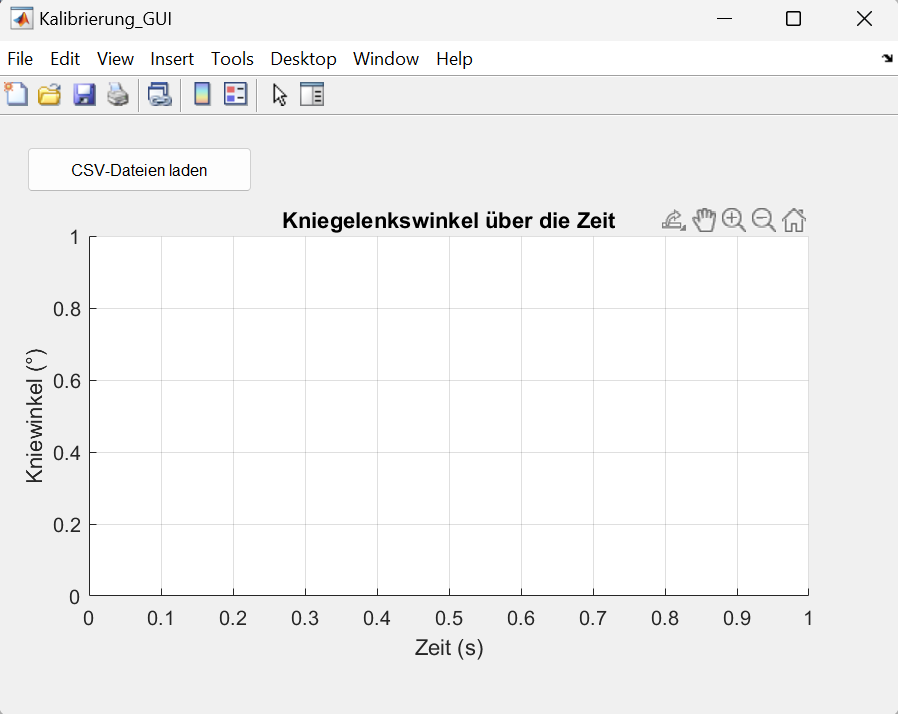
\includegraphics[width=0.75\linewidth]{images/Kalibrierung_GUI.png}
\caption{Oberfläche der Kalibierungs GUI}
\label{fig:Kalibrierungs GUI}
\end{figure}
\newpage
\subsubsection{Ablauf des Matlab-Programm KniewinkelAnalyse\_GUI}
\noindent Im Folgenden ist der Programmablaufplan der Kniewinkel-Analyse-GUI dargestellt. Die einzelnen Funktionen werden anschließend detailliert erklärt.

\noindent Die Kniewinkel-Analyse-GUI dient der Analyse des Kniegelenkwinkels anhand von CSV-Dateien. Die GUI besteht aus drei aufeinanderfolgenden Fenstern. Das erste GUI-Fenster ermöglicht die Auswahl der Kniebeugentiefe sowie die Eingabe der Probanden-ID.

\noindent Nach Betätigung des OK-Buttons wird die Callback-Funktion InfoGUI aufgerufen. In dieser Funktion werden die Informationstexte zu den verschiedenen Auswahlmöglichkeiten integriert sowie die Schwellenwerte gesetzt. Die Informationen zu den Schwellenwerten, der Probanden-ID und der ausgewählten Kniebeugen-Art werden anschließend an die nächste Funktion übergeben.

\noindent Für das dritte GUI-Fenster werden zunächst die Figur und die zugehörigen Komponenten erstellt.

\noindent Die verschiedenen Buttons sind mit Funktionen verknüpft. Zunächst wird der Button „CSV-Dateien laden“ betätigt, woraufhin die Funktion loadCSVCallback aufgerufen wird. Diese Funktion beinhaltet die gleichen Code-Komponenten wie die entsprechende Funktion in der Kalibrierung\_GUI.

\noindent Die Funktion SliderCallback setzt die Slider entsprechend des ausgewählten Schwellenwerts und speichert diesen, um ihn im weiteren Verlauf verwenden zu können.

\noindent Die Funktion updatePlot wird verwendet, um den Verlauf des Kniegelenkwinkels über die Zeit darzustellen. Zudem werden durch diese Funktion die gestrichelten Linien der Schwellenwerte eingefügt sowie die Minima bzw. die maximale Tiefe der Kniebeuge identifiziert. Hierfür wird die vorgefertigte MATLAB-Funktion findpeaks eingesetzt.

\begin{lstlisting}[style=Matlab-editor]
[~, locs] = findpeaks(-kniewinkel, 'MinPeakDistance', 130, 'MinPeakProminence', 25);
valid_times_minima = common_time(locs);
valid_minima = kniewinkel(locs);
\end{lstlisting}
\\
\noindent Die Anzahl der Kniebeugen innerhalb und außerhalb der Schwellenwerte wird zusätzlich berechnet und farblich im Plot markiert. Außerdem erfolgt eine Berechnung des durchschnittlichen Kniewinkels anhand der Minima, wozu die vorgefertigte MATLAB-Funktion mean verwendet wird.
\begin{lstlisting}[style=Matlab-editor]
average_minimum = mean(valid_minima);
\end{lstlisting}
\\
\noindent Zusätzlich gibt es ein Infofeld, in dem Informationen nach der Auswertung angezeigt werden. Dazu gehören die Probanden-ID, die Gesamtzahl der Kniebeugen, die Anzahl der Kniebeugen innerhalb der Schwellenwerte, die Anzahl der Kniebeugen oberhalb und unterhalb der Schwellenwerte sowie der durchschnittliche Kniegelenkswinkel.

\noindent Die letzte Funktion ist mit dem Speicher-Button verknüpft und heißt saveResultsCallback. Diese Funktion ermöglicht das Speichern der textlichen Rückmeldungen als Textdatei, wobei ein beliebiger Speicherort ausgewählt werden kann. Außerdem erfolgt eine Rückmeldung, ob das Speichern erfolgreich war oder nicht.
\begin{center}
\begin{tikzpicture}[node distance=1.4cm and 4cm, every node/.style={align=center}, >=stealth]

% Styles definieren
\tikzstyle{startstop} = [rectangle, rounded corners, minimum width=4.2cm, minimum height=1cm,text centered, draw=black, fill=gray!20]
\tikzstyle{KAG} = [rectangle, minimum width=5.0cm, minimum height=1.1cm, text centered, draw=black, fill=pink!20]
\tikzstyle{info} = [rectangle, minimum width=5.0cm, minimum height=1.1cm, text centered, draw=black, fill=yellow!10]
\tikzstyle{LMG} = [rectangle, minimum width=5.0cm, minimum height=1.1cm, text centered, draw=black, fill=purple!20]
\tikzstyle{load} = [rectangle, minimum width=5.0cm, minimum height=1.1cm, text centered, draw=black, fill=cyan!10]
\tikzstyle{save} = [rectangle, minimum width=5.0cm, minimum height=1.1cm, text centered, draw=black, fill=green!10]
\tikzstyle{plot} = [rectangle, minimum width=5.0cm, minimum height=1.1cm, text centered, draw=black, fill=blue!10]
\tikzstyle{schw} = [rectangle, minimum width=5.0cm, minimum height=1.1cm, text centered, draw=black, fill=orange!20]


% GUI-Teil
\node (start) [startstop] {Start Oberfläche mit Komponenten erstellen};
\node (auswahl) [KAG, below of=start] {Kniebeugen-Typ wählen};
\node (tiefe) [KAG, right=of auswahl, xshift=0.2cm] {Tiefe Kniebeuge};
\node (halbe) [KAG, below of=tiefe] {Halbe Kniebeuge};
\node (viertel) [KAG, below of=halbe] {Viertel Kniebeuge};
\node (spezial) [KAG, below of=viertel] {Spezielle Kniebeuge};

\node (id) [KAG, below of=auswahl] {Probanden-ID eingeben};
\node (OK) [KAG, below of=id] {OK Button}
\node (info) [startstop, below of=OK] {Info-Oberfläche};
\node (infotext) [info, below of=info] {Infotext anzeigen};
\node (schwelle) [info, below of=infotext] {Schwellwerte setzen};
\node (OK2) [info, below of=schwelle] {OK Button}
\node (start2) [startstop, below of=OK2] {Auswertung Oberfläche};
\node (3GUI) [LMG, below of=start2] {Komponenten erstellen und mit Funktionen verknüpfen};

% Hauptlinie
\node (csv) [load, below of=3GUI] {CSV-Dateien laden Button};
\node (schwell) [schw, below of=csv] {Schwellwerte übernehmen};
\node (plot) [plot, below of=schwell] {Kniewinkelverlauf + Schwellen + Minima plotten};
\node (auswertung) [plot, below of=plot] {Kniebeugen analysieren:\\ Anzahl und Bewertung};
\node (speichern) [save, below of=auswertung] {Auswertung als Text speichern};
\node (ende) [startstop, below of=speichern] {Ende};

% Rechte Abzweigung ab CSV-Dateien laden
\node (loadData) [load, right=of csv, xshift=0.01cm] {Daten einlesen mit \texttt{readtable}};
\node (syncAccel) [load, below of=loadData] {Zeit synchronisieren\\ über Beschleunigungsmaximum};
\node (calcAngle) [load, below of=syncAccel] {Neigungswinkel mit \texttt{atan2d}};
\node (interp) [load, below of=calcAngle] {Interpolation auf gemeinsamen Zeitvektor};
\node (kneeAngle) [load, below of=interp] {Kniewinkel berechnen};
\node (removeStart) [load, below of=kneeAngle] {Zeitraum $<$ 2s entfernen};

% Hauptflüsse
\draw [arrow] (start) -- (auswahl);
\draw [arrow] (auswahl) -- (tiefe);
\draw [arrow] (auswahl) -- (id);
\draw[arrow](id) -- (OK);
\draw [arrow] (tiefe) -- (halbe);
\draw [arrow] (halbe) -- (viertel);
\draw [arrow] (viertel) -- (spezial);
\draw [arrow] (OK) -- (info);
\draw [arrow] (info) -- (infotext)
\draw [arrow] (infotext) -- (schwelle);
\draw[arrow] (schwelle) -- (OK2)
\draw [arrow] (OK2) -- (start2);
\draw [arrow] (start2) -- (3GUI);
\draw[arrow] (3GUI) -- (csv)
\draw [arrow] (csv) -- (schwell)
\draw [arrow] (schwell) -- (plot);
\draw [arrow] (plot) -- (auswertung);
\draw [arrow] (auswertung) -- (speichern);
\draw [arrow] (speichern) -- (ende);

% Rechte Abzweigung von CSV
\draw [arrow] (csv) -- (loadData);
\draw [arrow] (loadData) -- (syncAccel);
\draw [arrow] (syncAccel) -- (calcAngle);
\draw [arrow] (calcAngle) -- (interp);
\draw [arrow] (interp) -- (kneeAngle);
\draw [arrow] (kneeAngle) -- (removeStart);

\end{tikzpicture}
\end{center}

\noindent Die Abbildung 9 zeigt die Oberfläche zur Auswahl des Kniebeugentyps. Über den Pfeil können die verschiedenen Optionen ausgewählt werden. Darunter kann im Textfeld die Probanden-ID eingegeben werden.
\begin{figure}[ht]\centering
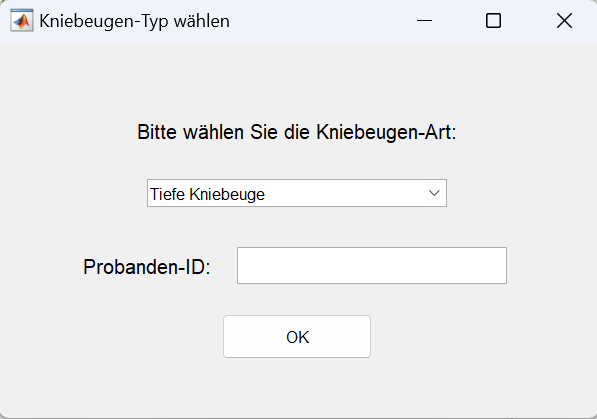
\includegraphics[width=0.75\linewidth]{images/Auswahl_GUI.png}
\caption{Oberfläche der Auswahl des Kniebeugentypes}
\label{fig:Kalibrierungs GUI}
\end{figure}
\noindent \noindent Die nächste Abbildung 10 zeigt die Oberfläche der Auswertungs-GUI. Oben links befindet sich der Button zum Laden der Daten. Rechts daneben werden die gesetzten Schwellenwerte angezeigt, welche bei Bedarf angepasst werden können.
\noindent Nach der Auswertung der Daten erscheint im darunterliegenden Diagramm der gemessene Winkelverlauf. Außerdem erfolgt oberhalb des Diagramms eine textliche Rückmeldung.
\noindent Über den oben rechts liegenden Button kann die textliche Auswertung, inklusive der Probanden-ID, als \texttt{.txt}-Datei abgespeichert werden.
\begin{figure}[ht]\centering
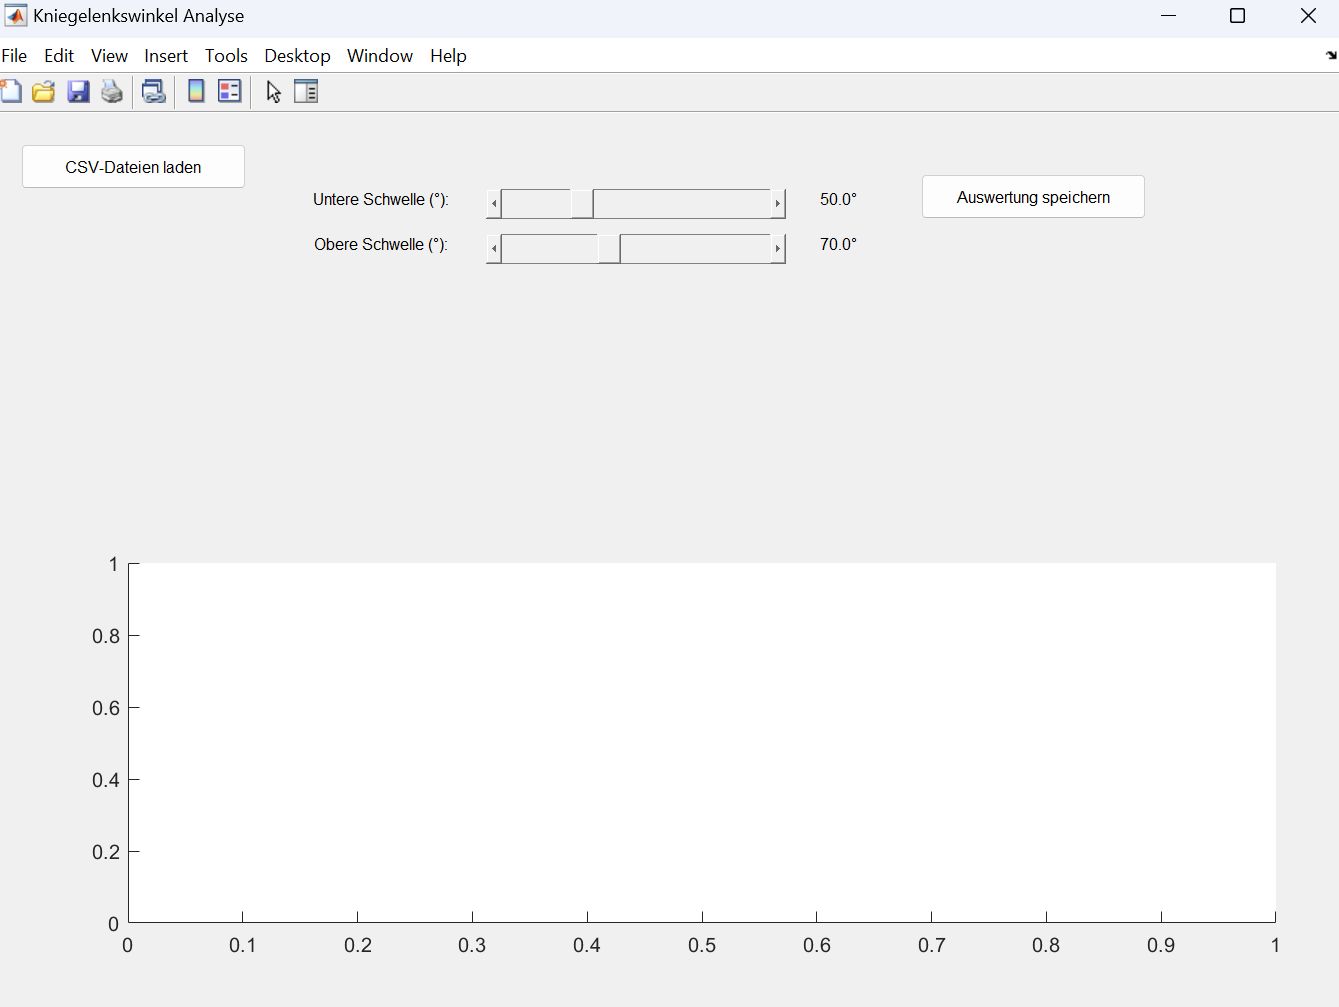
\includegraphics[width=0.75\linewidth]{images/Auswertungs_GUi.png}
\caption{Oberfläche der Auswertungs GUI}
\label{fig:Kalibrierungs GUI}
\end{figure}

\subsection{Versuchsdurchführung}
\noindent Im folgenden wird die Datenaufnahme in Phyphox und die anschließende Daten Auswertung erklärt. Anhand dieser Anleitung kann der Anwender Schritt für Schritt den Ablauf nachvollziehen und selber durchführen.

\noindent Das Ziel der entwickelten Anwendung ist die eigenständige Auswertung und Bewertung der Ausführung einer Kniebeuge hinsichtlich des Kniegelenkwinkels. Abhängig von verschiedenen Ausführungsvarianten wird bei der Kniebeuge ein unterschiedlicher Kniegelenkswinkel erwartet. 

\subsubsection{Einleitung und Zielsetzung}
Ziel des Versuchs ist die präzise Messung und Analyse des Kniegelenkwinkels bei der Durchführung von Kniebeugen mit unterschiedlichen Bewegungstiefen. Dabei soll überprüft werden, inwiefern die Versuchsperson die vorgegebenen Zielbereiche des Kniewinkels (tiefe, halbe und viertel Kniebeuge) einhalten kann. Die Auswertung erfolgt über eine eigens entwickelte MATLAB-GUI, die auf Basis der aufgezeichneten Sensordaten den Verlauf des Kniewinkels graphisch und textlich darstellt.

\subsubsection{Material und Geräte}
\begin{itemize}
    \item Beliebige Umgebung möglich
    \item 2x Smartphones mit installierter Phyphox-App
    \item 1x Smartphone mit Videokamera
    \item 1x Stativ zur Kamerapositionierung
    \item Befestigungsgurte zur Fixierung der Smartphones an Unter- und Oberschenkel
    \item Sporttape zur Befestigung
    \item 1x Winkelmesser
    \item 1x Stuhl, höhenverstellbar
    \item PC mit installierter Analyse-Software (KnieAngleGUI)
\end{itemize}

%% Für die GUI auch Links hinzufügen um die Runterzuladen 

\subsubsection{Technische Vorbereitung}
Für die Durchführung des Versuchs werden drei Smartphones benötigt, von denen zwei mit der Phyphox-App ausgestattet sind. Diese Geräte dienen der Messung der Beschleunigung an Oberschenkel und Unterschenkel. Das dritte Smartphone wird zur Videoaufzeichnung eingesetzt. Zusätzlich wird ein PC mit der installierten Auswertungssoftware benötigt. Vor Beginn des Versuchs werden alle Geräte eingeschaltet, die Phyphox-App vorbereitet und das Videoaufnahmegerät startklar gemacht. Der PC wird hochgefahren, sodass im Anschluss die aufgezeichneten Daten verarbeitet werden können.

\subsubsection{Vorbereitung der Versuchsperson}
Vor Beginn der Messung wird das schriftliche Einverständnis der Versuchsperson eingeholt. Zusätzlich werden mögliche gesundheitliche Einschränkungen oder bekannte Pathologien erfragt, um potenzielle Risiken auszuschließen. Die Versuchsperson sollte enganliegende oder kurze Kleidung tragen, insbesondere an den Beinen, um eine möglichst körpernahe Befestigung der Smartphones zu gewährleisten und Störfaktoren zu minimieren. Im Anschluss wird der Ablauf des Versuchs kurz erläutert. (Weitere Details siehe Anhang: Probandenaufklärung zur Studie „Messung des Kniegelenkwinkels bei Kniebeugen mit verschiedenen Anforderungen“.)

\subsubsection{Versuchsaufbau}
Die Länge des Beins bis zum Knie wird gemessen, um den Stuhl auf die passende Höhe einzustellen. Anschließend werden die beiden Mess-Smartphones mit Befestigungsgurten am Bein fixiert. Ein Smartphone wird seitlich am Oberschenkel, das andere seitlich am Unterschenkel angebracht. Die genaue Platzierung platzierung der Smartphone ist von Bedeutung um eine korrekte Analyse zur erhalten. Die genauen Befestigungspunkte werden anhand der Abbildung ?? dargestellt. 
\\
\\
?????? Bild von der Befestigung
\\
\\
Vor Beginn der Datenaufnahme sollte überprüft werden, ob die Smartphones fest sitzen und keine Bewegungseinschränkung verursachen.
\noindent Das dritte Smartphone wird auf einem Stativ in der Sagittalebene auf Höhe des Knies positioniert, um die Bewegung aufzuzeichnen.

\subsubsection{Kalibrierungsmessung}
\noindent Um die Daten der Phyphox-App korrekt auszuwerten, sollten vor der Aufnahme einige Vorbereitungen getroffen werden. Zur Kalibrierung wird zunächst ein Video gestartet und beide Phyphox-Apps geöffnet. Unter dem Sensor-Menüpunkt „Beschleunigung mit g“ wird die Messung möglichst gleichzeitig gestartet. Das Starten der Aufnahme erfolgt über den *Play*-Button in der oberen orangenen Leiste. Dies kann entweder von der Testperson selbst oder von einer helfenden Person durchgeführt werden. Falls das annähernd gleichzeitige Starten nicht gelingt, kann der Datensatz einfach über das "Mülltonnen-Symbol" gelöscht und die Aufnahme erneut gestartet werden. Sobald die Aufnahme läuft, kann die Durchführung der Übung beginnen.
\noindent Um beide Datensätze bei der Auswertung synchronisieren  zu können, sollte zu Beginn einen markanter Punkt in den Daten sichtbar sein. Am einfachsten ist es, das Bein einmalig ruckartig nach oben zu Bewegung. Dieser Ruck kann im Programm in beiden Datensätzen erkannt werden und ermöglicht so die exakte Synchronisierung. Danach setzt sich die Person ruhig auf den zuvor eingestellten Stuhl. 
\noindent Der Kniewinkel im Sitzen wird mit einem Winkelmesser überprüft und bei Bedarf manuell korrigiert, bis ein Winkel von 90° erreicht ist. Die Person bleibt etwa 10 Sekunden lang ruhig in dieser Position. Anschließend wird die Messung pausiert und das Video gestoppt.
\noindent Die aufgezeichneten Sensordaten werden als CSV-Dateien im Format „Comma, decimal point“ exportiert und sinnvoll benannt (z.B. Probemessung\_---\_1\_Oberschenkel). Die Daten werden auf dem Laptop gespeichert und in der KnieAngleGUI geladen. Dort erfolgt eine automatische Synchronisation und Berechnung des Kniewinkels. Liegt dieser nicht im Bereich von 90° ±5, wird die Kalibrierung durch erneutes Anpassen der Smartphone-Positionen wiederholt.

\subsubsection{Versuchsdurchführung}
\noindent Die Versuchsperson führt nacheinander drei Kniebeugenserien mit unterschiedlicher Zieltiefe durch:
\begin{itemize}
    \item Tiefe Kniebeugen (Kniewinkel zwischen 40° und 60°)
    \item Halbe Kniebeugen (Kniewinkel zwischen 80° und 100°)
    \item Viertel Kniebeugen (Kniewinkel zwischen 110° und 140°) \cite{Hartmann2014}
\end{itemize}
\noindent In den folgenden Abbildungen wird die Ausführungstiefe der verschiedenen Ausführungsvarianten Bildlich dargestellt. 
\\
\\
?????? Bilder für die Ausführungstiefe
\\
\\
\noindent Für jede der drei Serien (tiefe, halbe und viertel Kniebeuge) wird ein einheitlicher Ablauf durchgeführt. Zunächst wird das Video auf dem dritten Smartphone gestartet, und die aktuelle Uhrzeit wird notiert, um eine eindeutige Zuordnung der Daten zu ermöglichen. Anschließend wird auf beiden Phyphox-Geräten die Messung gleichzeitig gestartet. Zur Synchronisation der Sensoraufzeichnungen mit dem Video führt die Versuchsperson erneut einen kurzen Ruck mit dem Bein aus.
\noindent Daraufhin werden zehn Kniebeugen in der jeweils vorgegebenen Zieltiefe durchgeführt. Nach Abschluss der Bewegungsausführung sollte die Testperson ruhig stehen bleiben und die Messung wird  über die Phyphox-App gestoppt und das Video beendet. Die dabei aufgezeichneten Sensordaten werden anschließend als CSV-Dateien im Format „Comma, decimal point“ exportiert. Dazu wird in der oberen orangenen Leiste das Drei-Punkte-Menü ausgewählt. Nun kann eine Aktion ausgewählt werden in diesem Fall der Datenexport. Es ist darauf zu achten, dass die Dateien eindeutig und nachvollziehbar benannt werden – zum Beispiel Tiefe\_---\_Oberschenkel oder Halbe\_---\_Unterschenkel. Diese Dateien dienen als Grundlage für die spätere Auswertung in der Analyse-Software. 

\subsubsection{Datenauswertung}
\noindent Nach Abschluss aller Serien wird die KnieAngleGUI auf dem PC geöffnet. Dort wählt man die jeweilige Kniebeugenart aus und lädt die entsprechenden CSV-Dateien. Die Anwendung synchronisiert die Daten und berechnet den zeitlichen Verlauf des Kniewinkels.
\noindent Die Ergebnisse werden grafisch dargestellt. Kniebeugen, deren tiefster Punkt innerhalb des definierten Zielbereichs liegt, werden grün markiert. Abweichungen außerhalb des Zielbereichs erscheinen rot. Zusätzlich wird eine schriftliche Auswertung generiert, die folgende Informationen enthält: Gesamtanzahl der Kniebeugen, Anzahl der Kniebeugen innerhalb des Schwellwertbereichs, Anzahl der zu tiefen Kniebeugen, Anzahl der zu hohen Kniebeugen. 

\noindent (Weitere Details siehe Anhang: Versuchsprotokoll Kniebeugen) 

\subsubsection{Ergebnisse der Untersuchung}


\section{Limitationen}

\noindent Echtzeit!!!
\noindent Eventuell 2 Person zur Hilfe nötig
\noindent Umgang mit Computer sollte bekannt sein

\section{Ergebnisse der Studie in Bezug auf die vorangegangene Literatur}\label{sec:Auswertung}
\section{Fazit und Ausblick}\label{sec:Diskussion}

%\includepdf[pages=1-3]{Probandenaufklärung.pdf}

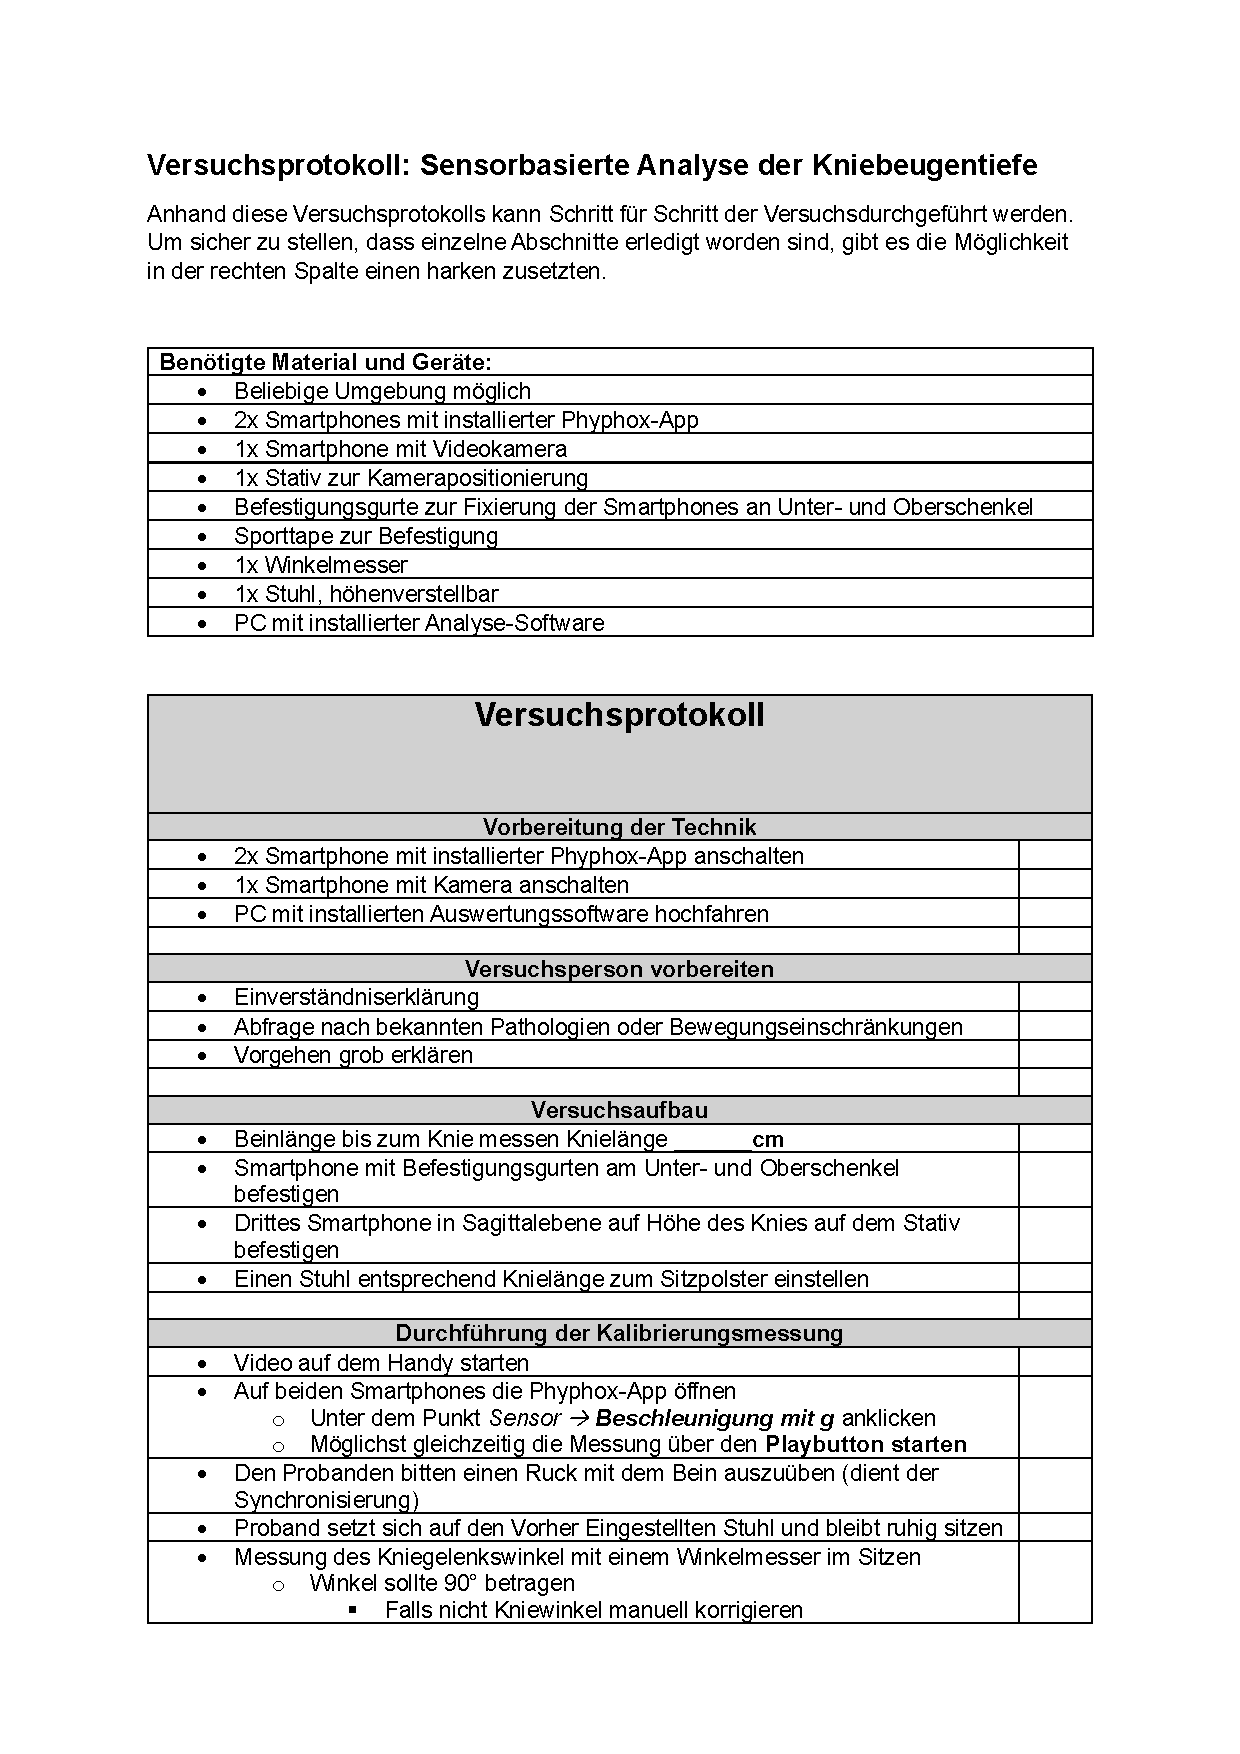
\includepdf[pages=1-3]{Versuchsprotokoll_Kniebeugen.pdf}
\newpage

\printbibliography % Einfügen der Bibliothek ins Dokument
\newpage

\appendix
%\section{Anhang}
\includepdf[pages=1-3]{Probandenaufklärung.pdf}

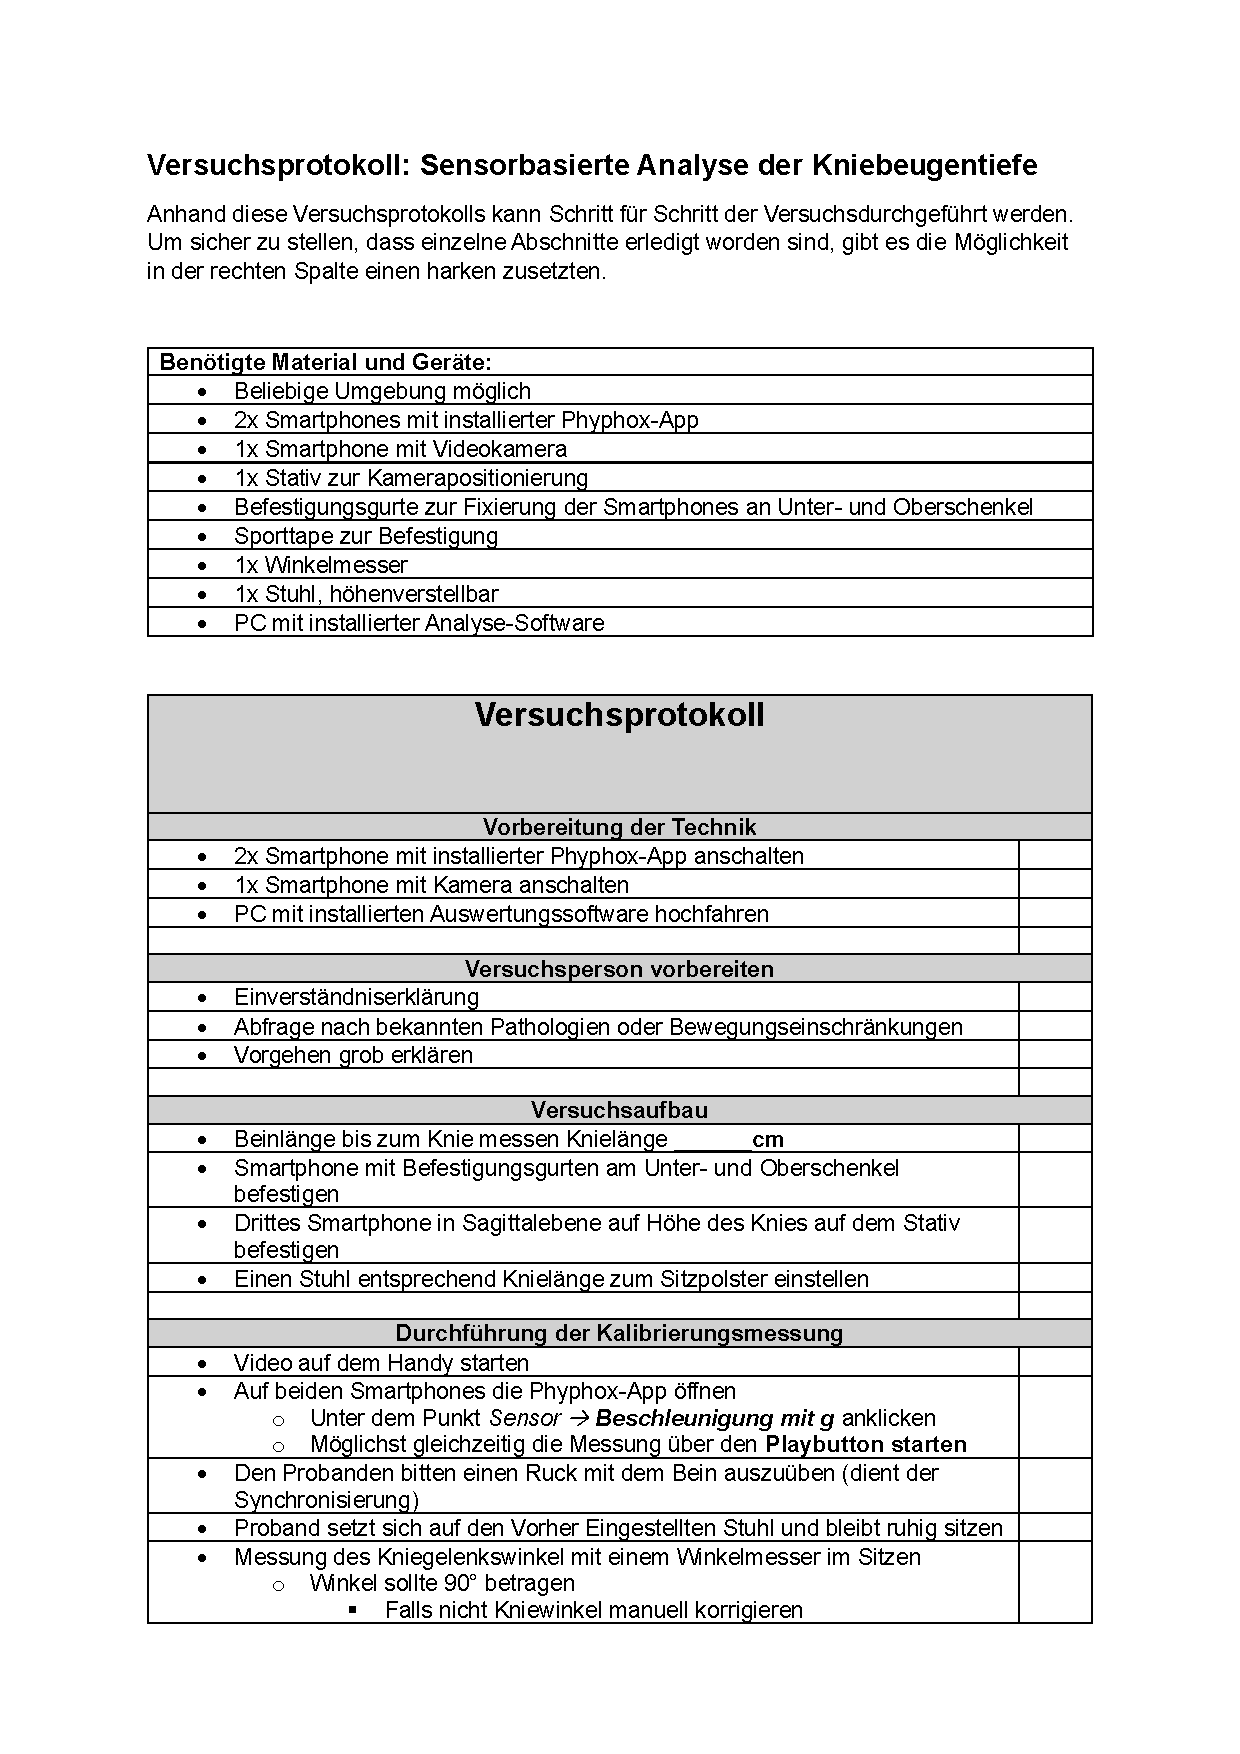
\includepdf[pages=1-3]{Versuchsprotokoll_Kniebeugen.pdf}

\end{document}